\documentclass[12]{article}
\usepackage[spanish,english]{babel}
%\usepackage[spanish]{babel}
\usepackage[utf8]{inputenc}
\usepackage{graphicx}
\usepackage{epsfig}
\usepackage{multirow}
\usepackage{multicol,caption}
\usepackage{amsthm} % Theorem Formatting
\usepackage{amssymb}    % Math symbols such as \mathbb
\usepackage{color}
\usepackage{hyperref}
\usepackage[none]{hyphenat}
\usepackage{appendix}
\usepackage{pdfpages}
\renewcommand{\appendixname}{Anexo}
\renewcommand{\appendixtocname}{LISTA DE ANEXOS}
\renewcommand{\appendixpagename}{Anexos}
%\renewcommand{\tablename}{Tabla}
%\def\tablename{Cuadro}% por \def\tablename{Tabla}% 
\newenvironment{Figure}
{\par\medskip\noindent\minipage{\linewidth}}
{\endminipage\par\medskip}
\addto\captionsspanish{%
\def\tablename{Tabla}%
}
\topmargin  = 10pt
\oddsidemargin  = -0.5in
%\headheight = 12pt
%\headsep    = 15pt
%\footskip   = 15pt
\textheight = 21.5 cm
\textwidth  = 18.5cm
\tolerance=10000
\title{\bf{Modulo motorizado para ilustrar la difracción, atenuación y absorción de ondas electromagnéticas en el espectro infrarrojo; utilizando tecnologías libres y de bajo costo.}}
\author{Diego Parra\footnote{diegoestudianteud1@gmail.com}, Julian Salamanca\footnote{jasalamanca@udistrital.edu.co} \\
  Universidad Distrital, Calle 3 No 26A-40 Bogotá-Colombia\\
  Grupo de Física e Informática ``FISINFOR''
}
\date{\today}
\begin{document}
%\def\tablename{Cuadro}% por \def \tablename{Tabla}% 
\renewcommand{\tablename}{Tabla}
\maketitle
\vspace{-0.8cm}
\selectlanguage{english}
\begin{abstract}

This writing describes in detail the construction of a motor vehicle taking advantage of the technological wonders of semiconductors to control hardware with a ATMEGA328P-Pu microcontroller with serial communication via Bluetooth to a computer whose operating system is GNU-Linux, equipped with a side infrared sensor illustrating the diffraction phenomenon and calculates the wavelength emitted by the lED diode emitting infrared; also it has a pair of emitter sensors - infrared receiver on the front of the vehicle, the infrared sensor front and infrared emitter front illustrate the law of decay density radiansa with the square of the distance to the radiating source, the reflectance and transmittance that occurs due to the interaction of the radiation with matter. \\\\
This project also has instructions for using the control software free infrarossi and their respective installation, whose function is to control the actions taken by the infrarossi vehicle, both forward and capture data from the side and front sensors and control the radiant source photon in the infrared, for examination. It is noteworthy that all this communication between the motor module infrarossi and control software comes pre designed to be via bluetooth.
{\bf{Keywords:}} infrarossi motorized module,  control software free infrarossi, law decay density radiansa with the inverse square, reflectance, diffraction, serial communication, bluetooth, GNU-Linux, software, hardware.
\selectlanguage{spanish}
\begin{center}
{\bf{Resumen}} 
\end{center}
  
El presente escrito, describe detalladamente la construcción de un vehículo motorizado  aprovechando las maravillas tecnológicas de los semiconductores para el control de hardware con un microcontrolador atmega328P-Pu, con comunicación serial vía bluetooth con un ordenador cuyo sistema operativo es GNU-Linux, equipado con un sensor  infrarrojo lateral que ilustra el fenómeno de difracción y calcula la longitud de onda emitida por el diodo led emisor en infrarrojo; también tiene un par de sensores emisor – receptor infrarrojo en la parte del frente del vehículo, el sensor infrarrojo frontal y el emisor infrarrojo frontal ilustran la ley del decaimiento de  la densidad de radiansa con el cuadrado de la distancia a la fuente radiante,  la reflectancia y  transmitancia que ocurre debido a la interacción de esta radiación con la materia.\\\\
Este proyecto cuenta también con las indicaciones para el uso del software de control free infrarossi y su respectiva instalación, cuya función es controlar las acciones que realiza el vehículo infrarossi, tanto  avanzar  y capturar datos de los sensores  lateral y frontal como de controlar la fuente radiante de fotones en el infrarrojo, para su respectivo análisis. Cabe mencionar que toda esta comunicación entre el modulo motorizado infrarossi y su software de control viene pre diseñada para que sea  vía bluetooth.
\\
{\bf{Descriptores:}}Modulo motorizado infrarossi, software de control free infrarossi, ley de decaimiento de la densidad de radiansa con el inverso del cuadrado, reflectancia, difracción, comunicación serial, bluetooth GNU-Linux, software, hardware.
\end{abstract}
%tabla de contenido sin numeracion
%\renewcommand\contentsname{\centering TABLA DE CONTENIDO}
%\thispagestyle{empty}
%\setcounter{page}{1}
%\tableofcontents
%\clearpage
%lista de figuras
%\renewcommand\listfigurename{\centering LISTA DE FIGURAS}
%\listoffigures
%\clearpage
%lista de tablas
% \renewcommand\listtablename{\centering LISTA DE TABLAS}
% \listoftables
% \clearpage
\begin{multicols}{2}
\section{Introducción}
En la actualidad, una cantidad de instrumentos de laboratorio para la enseñanza en física y especialmente de  fenómenos electromagnéticos,  transporte e inyección de energía a los portadores de carga en los semiconductores, portentos ondulatorios, etc.; son  muy costosos, incluso estos instrumentos son exclusivos de los departamentos de ciencias en diferentes  universidades y laboratorios, lo que dificulta el acercamiento de la población a estas manifestaciones físicas; un caso especial es el estudio de las propiedades de las ondas electromagnéticas y su dualidad onda – partícula, en determinadas frecuencias “caso clásico” o en paquetes de energía discreta según su longitud de onda “caso cuántico”; específicamente en cuestión de frecuencias o longitudes de onda que corresponden al espectro electromagnético infrarrojo, concretamente cuando se habla de difracción, atenuación, absorbancia, transmitancia, reflectancia,   ley de decaimiento de la densidad de radiansa con el inverso del cuadrado de la distancia a la fuente; solo se tiene como marco de estudio de estos portentos fenómenos ondulatorios infrarrojos a la espectrometría  infrarroja, que es usada habitualmente por estudiantes de medicina, química, biología, etc., muy especializados, con instrumentos muy costosos y precisos;  lo que deja sin aproximarse a los demás estudiantes de ciencias exactas a estos tópicos de la física que están presentes en la vida diaria y que no son visibles al ojo humano.\\\\
El objetivo de este trabajo de grado es diseñar un instrumento de laboratorio que sea capaz de ilustrar tres  portentos físicos  de la radiación electromagnética y su dualidad onda – partícula; los cuales son: difracción en infrarrojo, reflectancia en el infrarrojo y ley del decaimiento de la irradiansa con el inverso del cuadrado de la distancia a la fuente. Esto con el fin de dejar  referencia que en la actualidad no se estudia de manera cómoda los fenómenos ondulatorios y de interacción de esta manifestación física de la energía con la materia, en el espectro de está longitud de onda como lo es el infrarrojo. \\\\
Por esta razón se elabora muy cuidadosamente un instrumento que llene las expectativas de aprendices y docentes de carreras afines a  estos asuntos;  el cual es económico, con materiales de fácil acceso, que es capaz de aproximar al educando a portentos como lo es la difracción, la ley del decaimiento de  la densidad de radiansa con el inverso del cuadrado de la distancia a la fuente radiante,  la reflectancia y  transmitancia que ocurre debido a la interacción de esta radiación con la materia, en el rango infrarrojo del espectro.  \\\\
A este instrumento se le denomino $modulo$ $motorizado$ $infrarossi$, el cual es un vehículo de tracción electromagnética, con comunicación serial vía bluetooth con un ordenador GNU-Linux, equipado con un sensor infrarrojo lateral para ilustrar el fenómeno de difracción, un sensor infrarrojo frontal y un emisor infrarrojo frontal para ilustrar la ley del decaimiento de  la densidad de radiansa con el cuadrado de la distancia a la fuente radiante,  la reflectancia y  transmitancia que ocurre debido a la interacción de esta radiación con la materia; el modulo infrarossi es capaz de acercar de manera cualitativa y cuantitativa al estudio de estos contenidos, pues aparte del instrumento que obtiene los datos, también cuenta con un software de control   y análisis de datos obtenidos, a este software se le designo el nombre de $software$ $de$ $control$ $free$ $infrarossi$, el cual complementa el modulo motorizado infrarossi, convirtiéndolo en una herramienta de laboratorio muy precisa, económica, fácil de utilizar, con su propio repositorio en github, con buena  documentación, fácil de manipular e instalar.
\section{Diseño experimental}
El diseño elegido para este montaje es el de un vehículo de tracción electromagnética, con cuatro ruedas,  dos delanteras y dos traseras, se ubicara (visto desde las ruedas traseras) un diodo receptor infrarrojo en la parte lateral derecha, un diodo emisor y otro receptor infrarrojo en la parte frontal del vehículo, todos los sensores deben quedar a una distancia de seis  centímetros  del suelo, cuenta también con un microcontrolador atmega 328 P-PU que es el encargado de controlar los sensores infrarrojos, el diodo emisor infrarrojo y la distancia que debe avanzar el vehículo; la comunicación del vehículo con el ordenador se realiza con un modulo bluetooth hc-05, el cual tiene como tarea principal informarle al microcontrolador atmega 328 P-PU las ordenes que debe realizar, dispuestas por el investigador y enviadas por el ordenador al dispositivo bluetooth.\\\\
Utilice todas las medidas de seguridad al momento de manipular las herramientas para moldear este proyecto; a continuación se detalla su elaboración.
\subsection{ Materiales para el montaje}
\begin{enumerate}
\item[a.] Un ordenador con sistema operativo GNU-Linux\footnote{Se utilizo ordenador toshiba satellite skullcandy con sistema operativo linux mint 17.2}.
\item[b.] Microcontrolador atmega\footnote{Para realizar la parte de control del hardware.} 328P-PU \cite{ARDUINO}.
\item[c.] Dos diodos led infrarrojos receptores de $5 mm$.
\item[d.] Un diodo led infrarrojo emisor de dimensiones  $5.0$x$7.6 mm$, de longitud de onda $\lambda = 940 nm $,  el cual tiene un color estándar agua clara.
\item[e.] Un motor de 9 voltios DC con sistema de engranajes de eje móvil\footnote{Para el movimiento del vehículo.}.
\item[f.] Modulo Bluetooth\footnote{Permite la comunicación a distancia con el dispositivo, sin necesidad de un sistema físico cableado.} HC-05.
\item[g.] Transistor\footnote{Es transformador de voltaje de 9 voltios a 5 voltios el cual alimentara el microcontrolador atmega328P-PU, y los demás dispositivos.} LM-7805CV \cite{REGULADOR}.
\item[h.] Un cristal de 16 MHz.
\item[i.] Tarjeta arduino \cite{ARDUINO} uno.
\item[j.] Tres resistencias de 500 ohms.
\item[h.] Dos resistencia de 3k$\Omega$.
\item[i.] Tres resistencias de 1 k$\Omega$.
\item[j.] Diodo rectificador de referencia 1N4001. 
\item[k.] Dos capacitores cerámicos de 12 picofaradios.
\item[l.] Dos capacitores de 10 microfaradios.
\item[m.] Transistor TIP\footnote{Control de la rapidez de giro del motor.} 122\cite{TIP122}  
\item[n.] Cuatro llantas de 2.5 cm de radio y 2 cm de ancho.
\item[ñ.] Una batería de 9 V.
\item[o.] Una lamina de madeflex, triplex  o un acrílico de 14x12x0.3 $cm^{3}$
\item[p.] Un interruptor pequeño.
\item[q.] Tres diodos led de cualquier color, o un diodo rgb de ánodo común.
\item[r.] Base 28 pines para microcontrolador.
\end{enumerate}
\subsection{Montaje eléctrico}
En esta sección se explica como deben ir conectadas las diferentes partes eléctricas que  abarca el vehículo motorizado free infrarossi. Soldar primero la base de 28 pines del microcontrolador, a una tarjeta de circuito perforada, esto con el fin que el microcontrolador quede libre para programarlo y montarlo en la base nuevamente al final del proyecto. Las imágenes de los montajes se realizó en en fritzing\footnote{Enlace a la pagina oficial del proyecto fritzing http://www.fritzing.org/home/}. Tenga en cuenta que este proyecto se pensó para realizarlo en dos tarjetas de circuitos electrónicos, en la primer tarjeta se conecto el transformador de $9 V$ a   $5 V$, el oscilador, la base de 28 pines para el microcontrolador\footnote{Tenga en cuenta el sentido de la base para conectar el microcontrolador, pues las conexiones deben hacerse en los pines indicados.}, el modulo bluetooth HC-05 y el botón reset; en la segunda tarjeta se acoplan los sensores infrarrojos\footnote{En la disposición prevista en el primer párrafo del diseño experimental}, el control de velocidad del motor y los diodos led de colores. \footnote{Los esquemas de las figuras  1-4 y 6 pertenecen a la pagina principal del proyecto arduino\cite{ARDUINO}, y modificadas en fritzing\cite{FRITZING}.}.
\subsubsection{Transformador de 9 a 5 Voltios}
Estructura del transformador de 9 voltios a 5 voltios, se realiza con dos capacitores electrolíticos de 10 microfaradios  y el transistor lm7805cv\cite{REGULADOR}. Ambos  capacitores deben ir en paralelo quedando su extremo negativo conectado a tierra y su extremo positivo uno a la entrada de 9 V y el otro a la salida de 5 V del transistor, el transistor lm consta de 3 pines uno de los cuales es la entrada de +9V, el pin de la mitad es tierra o GND y el pin extremo es la salida a 5V; tal como se muestra en la figura 1.A; en la figura 1.B se coloco un enchufe para la batería. 
\selectlanguage{spanish}
\begin{Figure}
\center
\begin{tabular}{|l|r|}
\hline
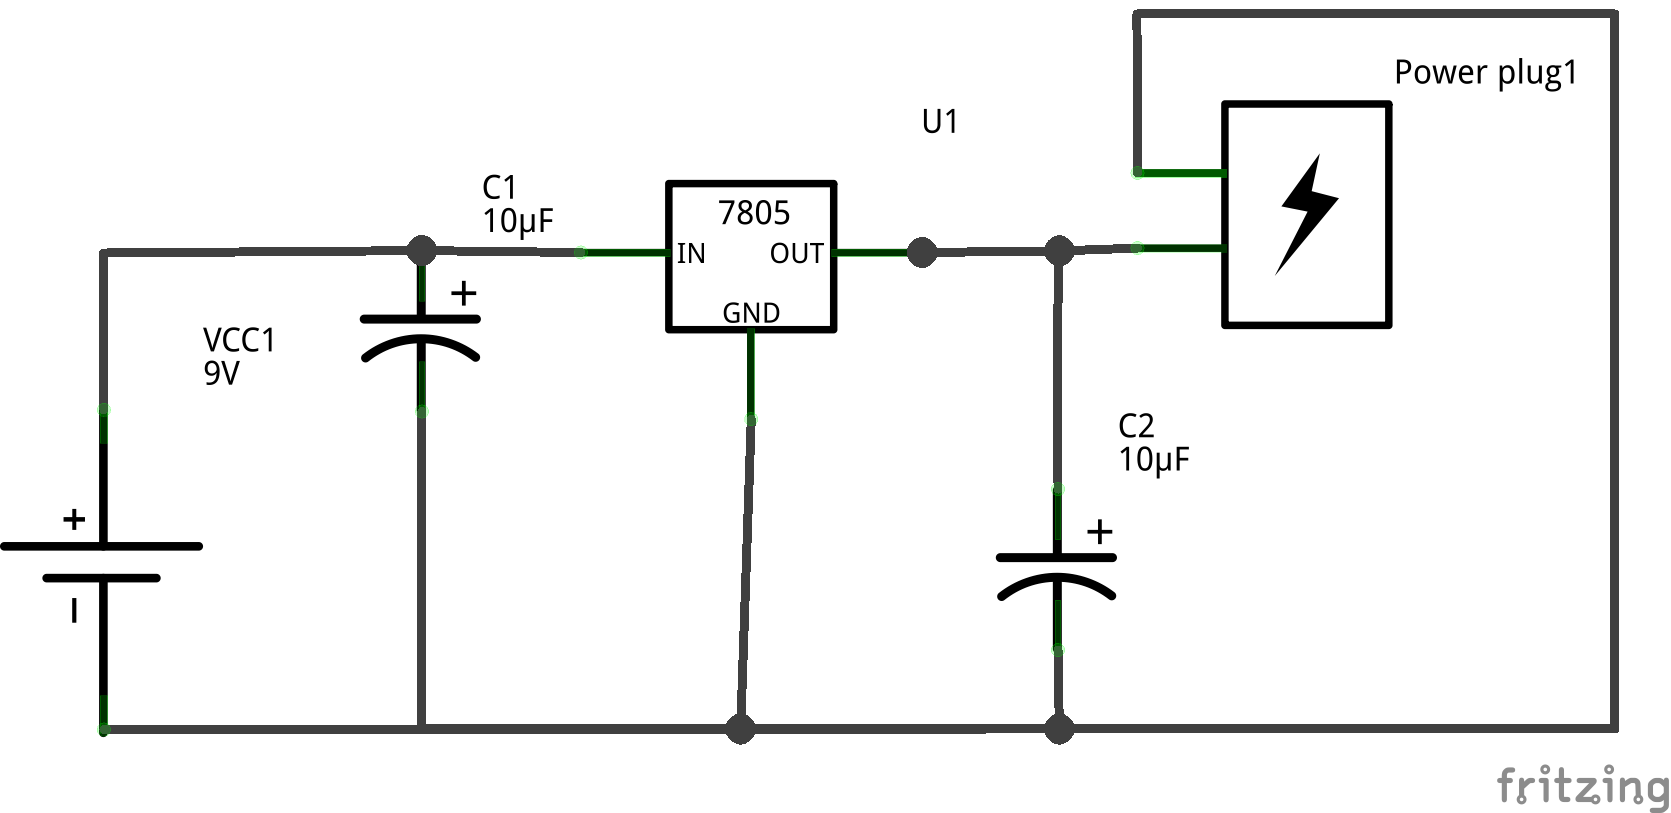
\includegraphics[width=4cm, height=4cm]{img/esquematrans.png}  & 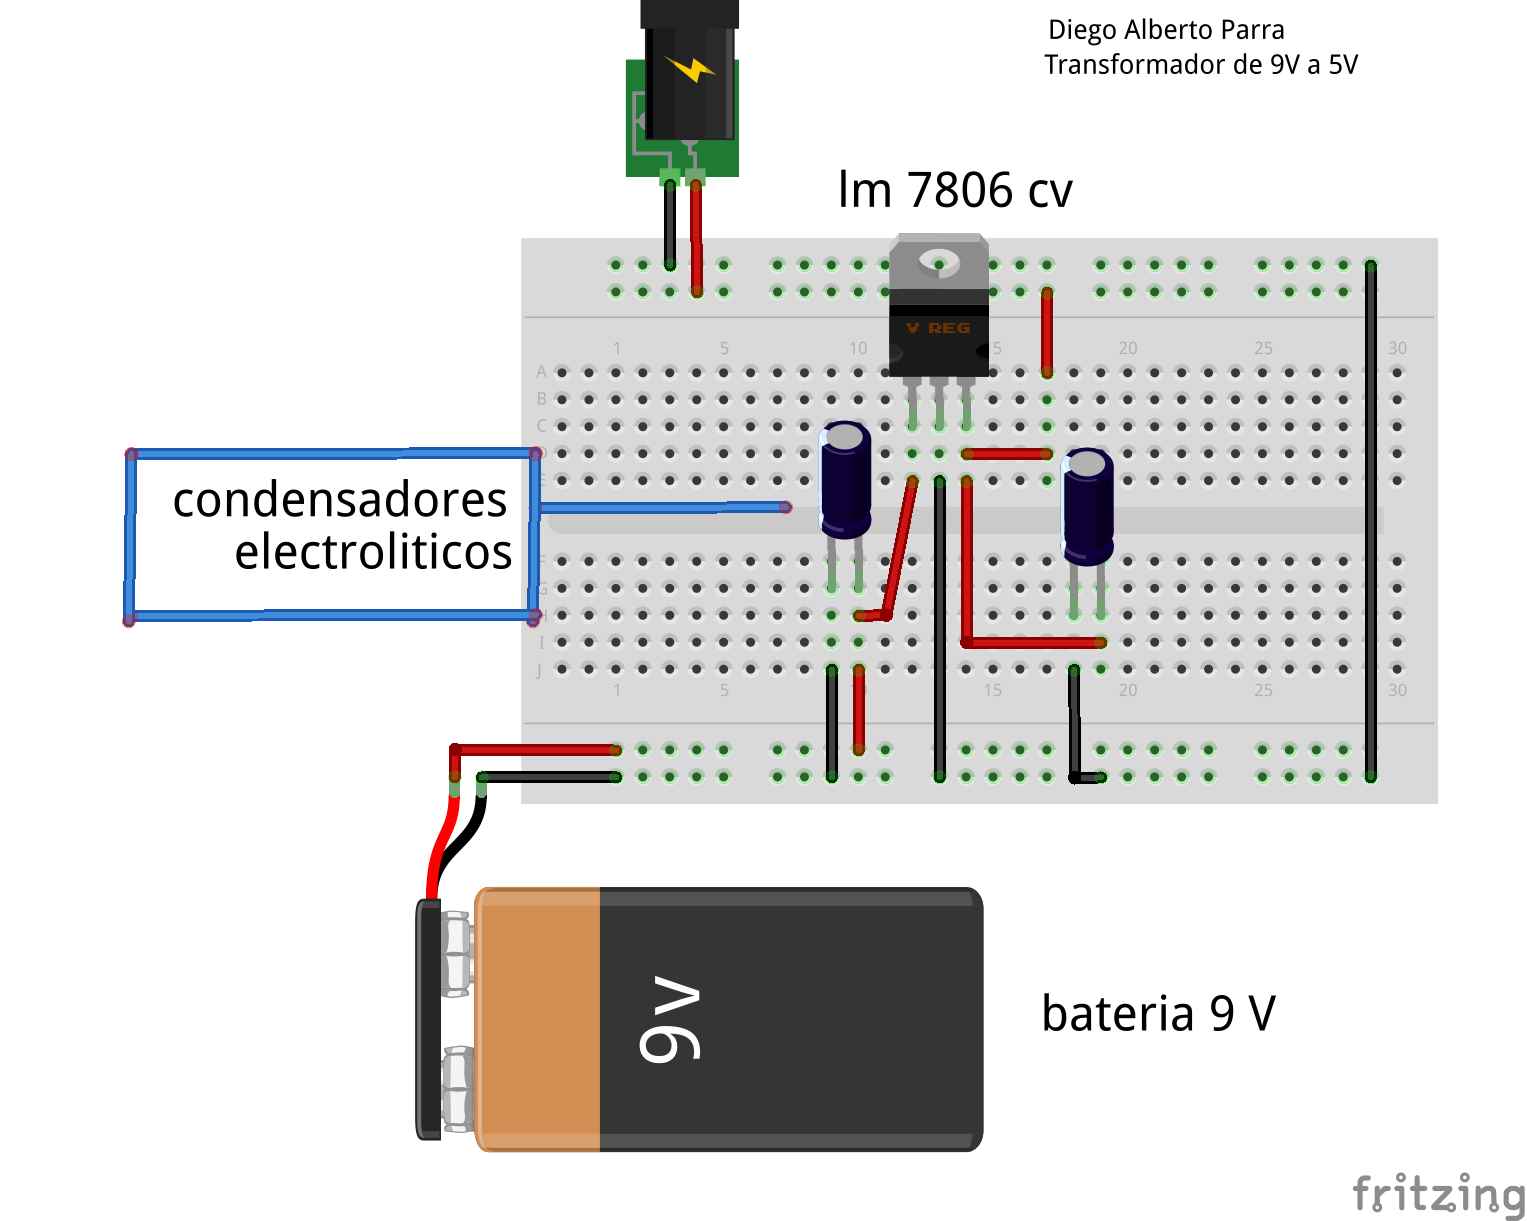
\includegraphics[width=4.cm, height=4cm]{img/montajetr5V.png} \\ \hline
1.A & 1.B \\ \hline
\end{tabular}
\captionof{figure}{Figura 1.A Esquema eléctrico del transformador\cite{REGULADOR} de 9V a 5V, con un transistor lm 7805 cv, dos capacitores electrolíticos de 10 microfaradios.  Figura 1.B Montaje en protoboard del circuito.}
\label{fig:g1}
\end{Figure}
\subsubsection{Modulo bluetooth}
El modulo bluetooth se debe conectar de la siguiente manera: el pin 2 de la tarjeta arduino es el Rx, este va conectado al Tx del bluetooth, el pin 3 del microcontrolador es el Tx y va conectado al pin Rx del bluetooth, como se muestra en la figura 2.A y 2.B, conectar el GND del bluetooth al pin 8  o 16 del microcontrolador, ahora conectar el pin de Vcc del bluetooth al pin 7 o 14 del microcontrolador.
\begin{Figure}
\center
\begin{tabular}{|l|r|}
\hline
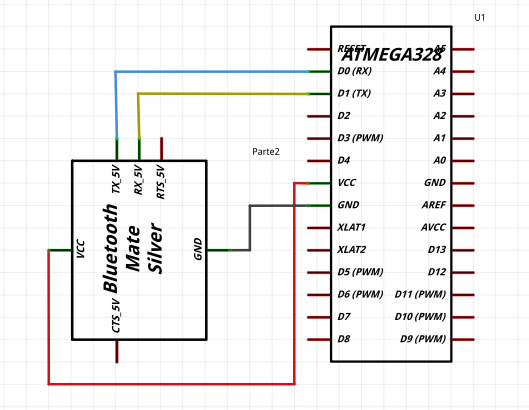
\includegraphics[width=4cm, height=4cm]{img/bluetoothesq.png} & 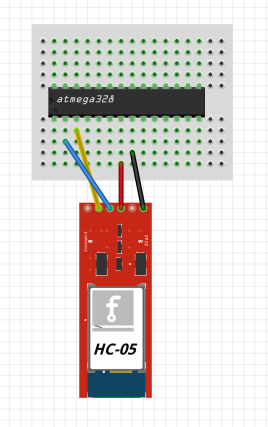
\includegraphics[width=4cm, height=4cm]{img/bluetoothmon.png} \\ \hline
2.A & 2.B \\ \hline
\end{tabular}
\captionof{figure}{Figura 2.A Circuito eléctrico del bluetooth conectado al microcontrolador. Figura 2.B Montaje en protoboard, los cables negros son tierra, los cables rojos son voltaje, y los cables de colores son conexiones.}
\label{fig:g2}
\end{Figure}
Esta es una pieza clave en el proyecto pues permite la comunicación a distancia con el microcontrolador y así de esta manera manipular el semiconductor para que avance, capture datos o simplemente suspenda todas las funciones y quede en reposo.
\subsubsection{Oscilador}
Es necesario colocar un oscilador de 16 mHz el cual se deja siempre en el microcontrolador, esto  con el fin de ajustar los tres relojes internos que trae el integrado atmega 328 P-Pu, para esto se utiliza el cristal de 16 mHz junto con los dos condensadores cerámicos de 12 picofaradios como se muestra en las figuras 3.A y 3.B, uno de los pines del cristal se conecta al pin 9 del microcontrolador y el otro extremo del cristal al pin 10, unir un capacitor a cada extremo del cristal y estos al pin 8 y 16 del microcontrolador de tal forma que los capacitores quedan en paralelo.\\
\begin{Figure}
\center
\begin{tabular}{|l|r|}
\hline
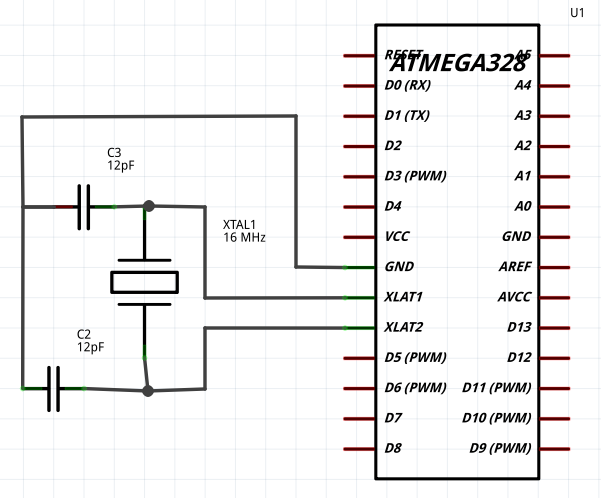
\includegraphics[width=4cm, height=4cm]{img/oscilaesq.png} & 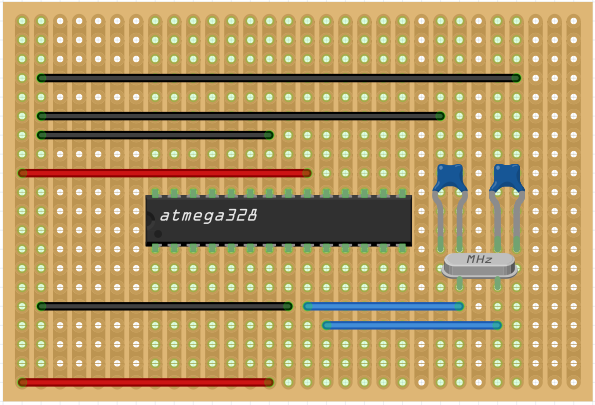
\includegraphics[width=4cm, height=4cm]{img/oscilapro.png} \\ \hline
3.A & 3.B \\ \hline
\end{tabular}
\captionof{figure}{Figura 3.A Esquema circuito eléctrico cristal 16 Mhz, conectado al microcontrolado. Figura 3.B Montaje en protoboard, los cables negros son tierra, los cables rojos son voltaje, y los cables de colores son conexiones.}
\label{fig:g3}
\end{Figure}
\subsubsection{Botón reset}
Se conecta un  botón como se muestra en la figuras 4.A y 4.B, para reiniciar el  microcontrolador, se une cualquiera de los  extremos del botón al pin 1 del microcontrolador que es el pin de reset, el otro extremo del botón se conecta  a una resistencia de 1 $K\Omega $ y el extremo de la resistencia a tierra.\\
\begin{Figure}
\center
\begin{tabular}{|l|r|}
\hline
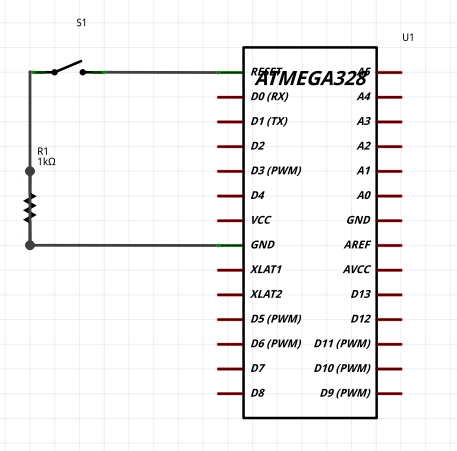
\includegraphics[width=4cm, height=3cm]{img/botonesq.png} & 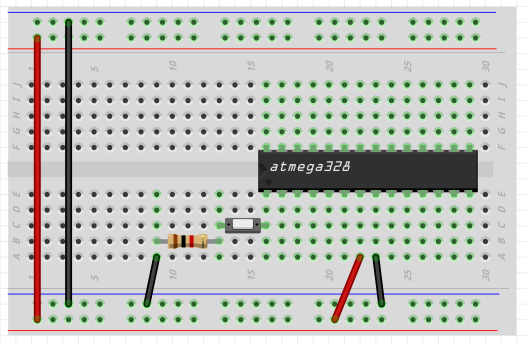
\includegraphics[width=4cm, height=3cm]{img/botonpro.png} \\ \hline
4.A & 4.B \\ \hline
\end{tabular}
\captionof{figure}{Figura 4.A Esquema conexión botón y microcontrolador atmega 328 P-PU. Figura 4.B Montaje en protoboard, los cables negros son tierra, los cables rojos son voltaje.}
\label{fig:g4}
\end{Figure}
\subsubsection{Control de velocidad del motor}
Conectar el motor y un sistema de transmisión como se aprecia en la figura 5; se utiliza un transistor tip\cite{TIP122} 122, las conexiones del transistor se muestran en la  figuras 6.A y 6.B.
\vspace{2cm}
Conectar una resistencia de 1 $k \Omega $ al pin base del transistor y el otro extremo de la resistencia\footnote{Esto con el fin de limitar la corriente de saturación que llega al pin  base del TIP122 que es de 2 mA a 20 mA, pues el pin PWM del integrado atmega 328 ofrece de 0 a 40 mA de salida.}  unido al pin numero 5 del integrado atmega328P-PU, luego conectar el pin del colector del tip122 a +5V, conectar un  diodo\footnote{El cual se encargara de limitar la corriente en caso de retornar por el colector del transistor hacia tierra cuando el motor se detenga.} regulador entre el colector y uno de los extremos del motor; unir el pin emisor del transistor  al extremo libre del motor y estos dos a tierra; ahora se conecta el condensador cerámico entre los dos pines del motor, como se observa en las  figuras 6.A y 6.B.\\\\
\begin{Figure}
\center
\begin{tabular}{|l|r|}
\hline
\\
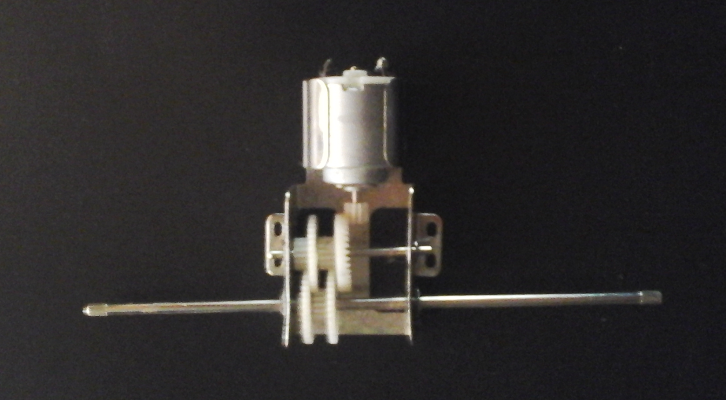
\includegraphics[width=6cm, height=4cm]{img/transmision.png}  \\\\ \hline
\end{tabular}
\captionof{figure}{Motor con sistema de transmisión para el montaje.}
\label{fig:g5}
\end{Figure}
\vspace{0.5 cm}
Tenga en cuenta que solo se conecta las terminales del motor, pues el sistema motor trasmisión deben ir ajustadas con tornillos debajo de la madera o el acrílico tal como se muestra en el anexo B-4.\\\\
\begin{Figure}
\center
\begin{tabular}{|l|r|}
\hline
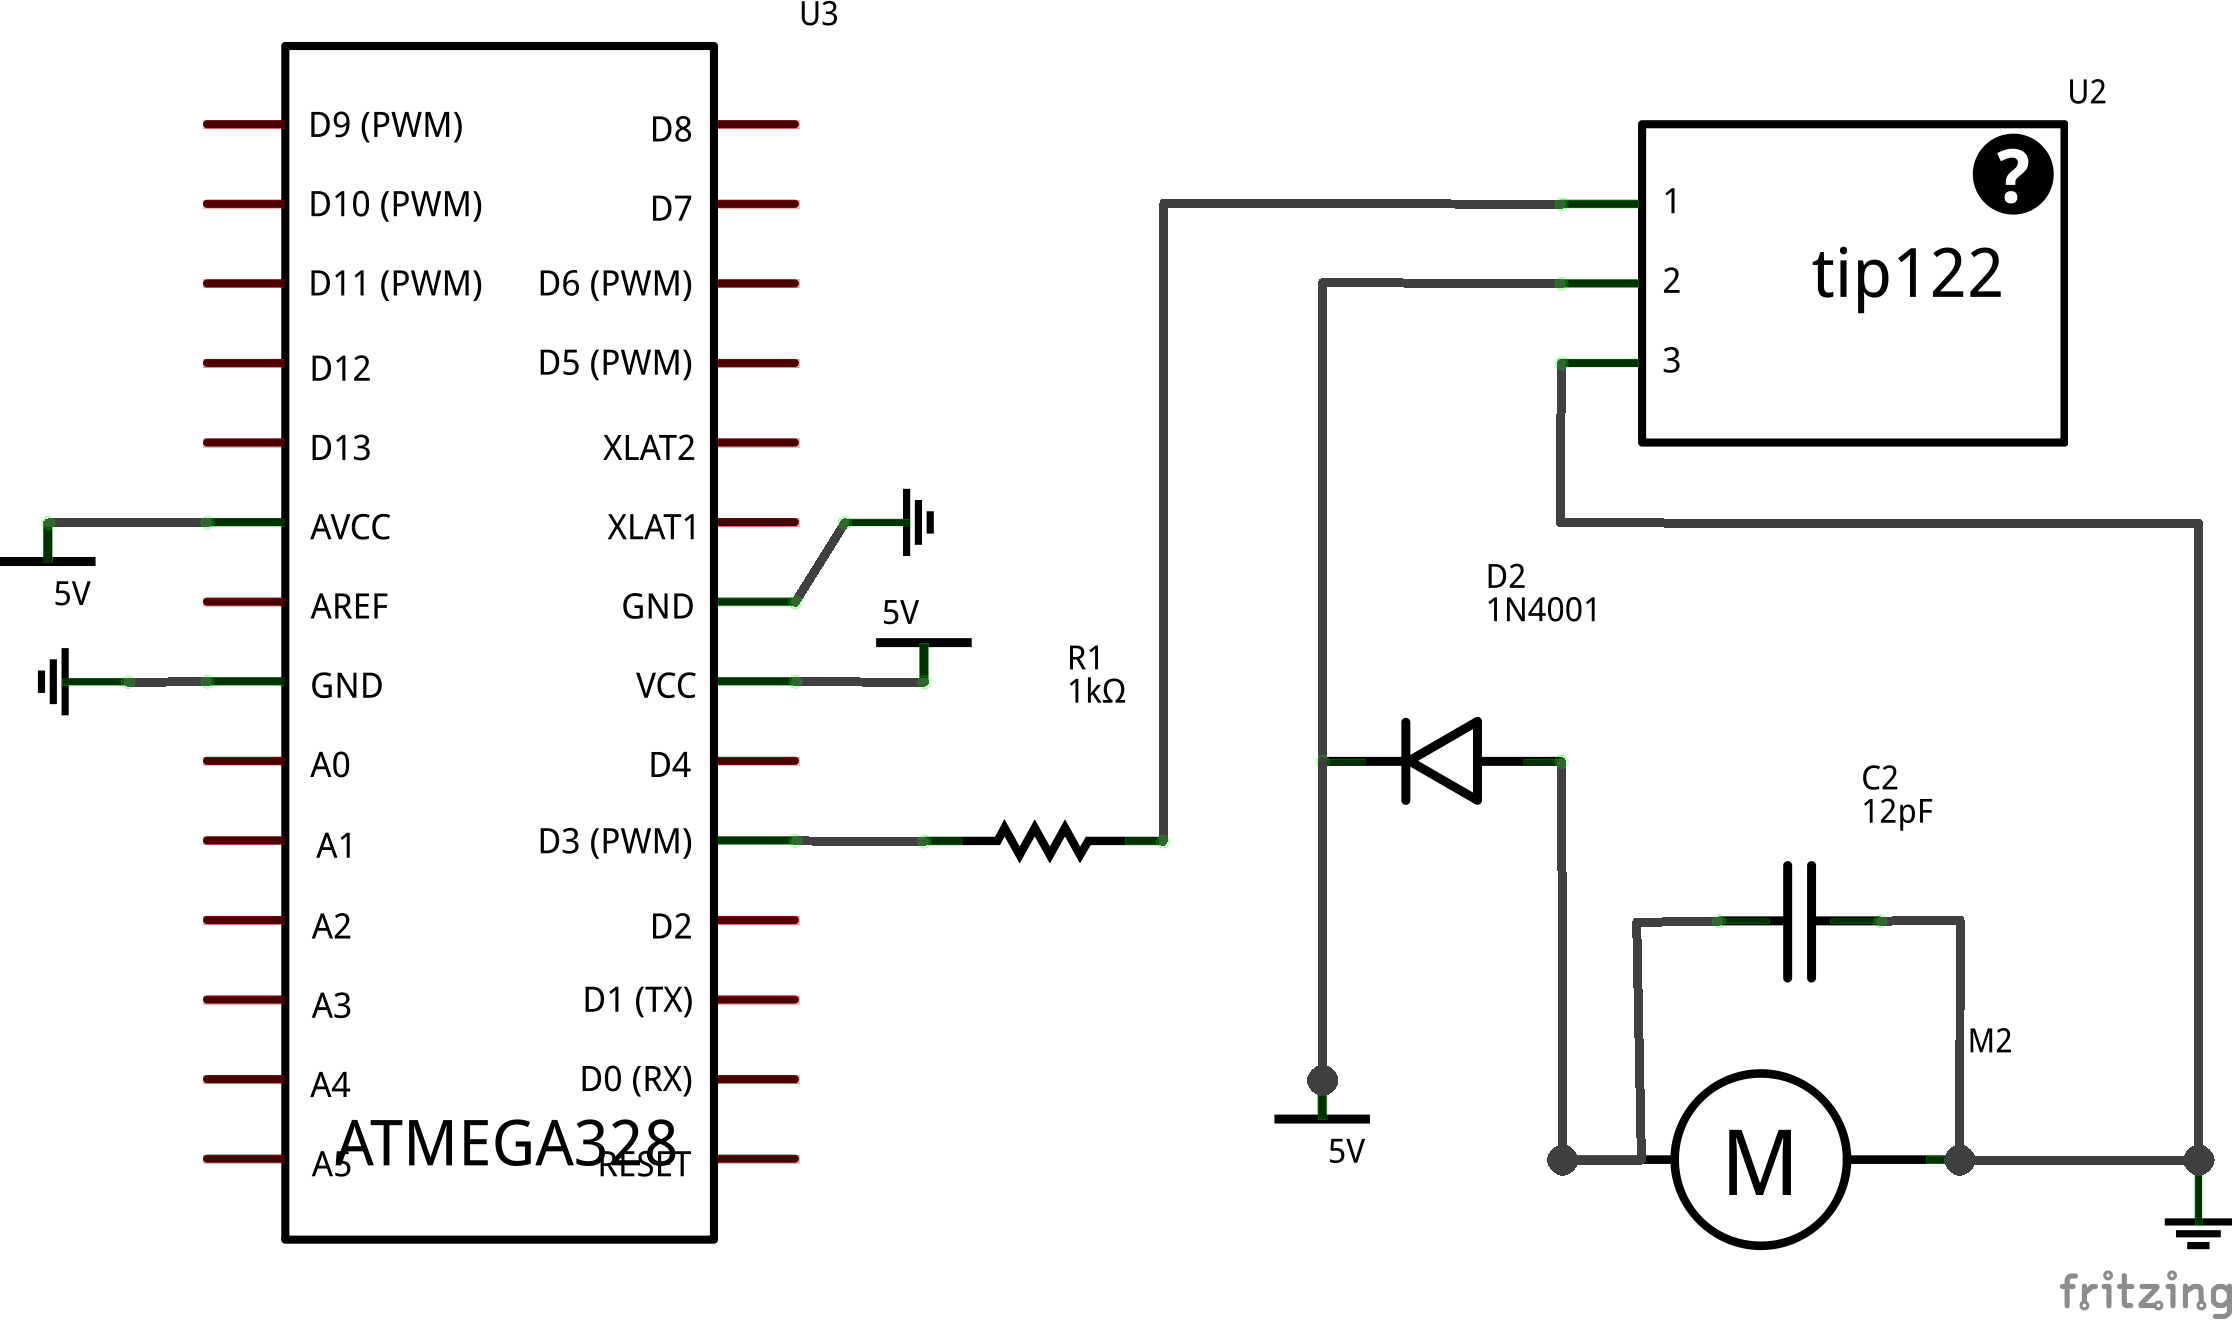
\includegraphics[width=4cm, height=3cm]{img/esquemamotor.png} & 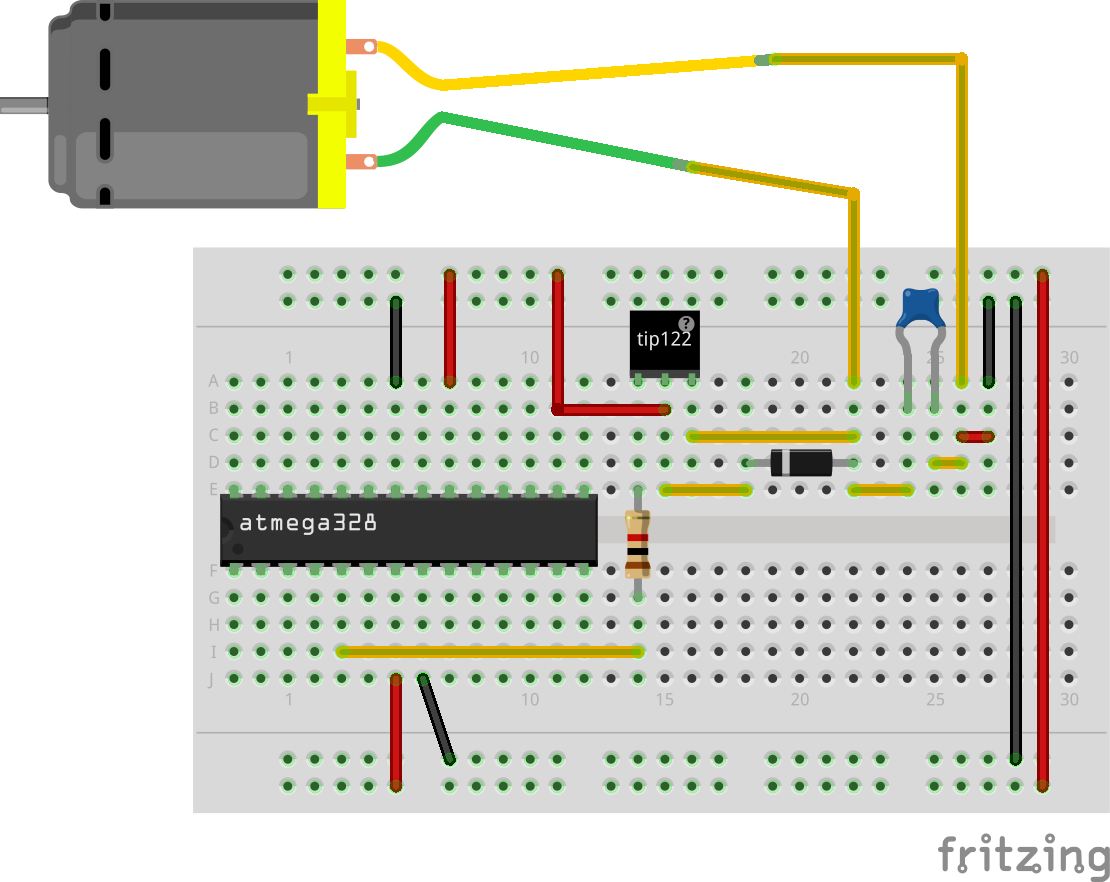
\includegraphics[width=4cm, height=3cm]{img/montajemot.png} \\ \hline
6.A. & 6.B. \\ \hline
\end{tabular}
\captionof{figure}{Figura 6.A Montaje eléctrico del motor conectado al microcontrolador, el tip 122, un diodo regulador, un capacitor cerámico de  12 pF y  resistencia de 1 Komhs. Figura 6.B Montaje en protoboard, los cables negros son tierra, los cables rojos son voltaje, y los cables naranjas son conexiones.}
\label{fig:g6}
\end{Figure}
\subsubsection{Sensor receptor lateral}
Las conexiones del sensor receptor lateral, el cual es un diodo led receptor de luz infrarroja; se conecta una resistencia de $3 k\Omega$ al ánodo del led y el otro extremo de la resistencia a tierra, luego se conecta el cátodo del led a $+5V$, el pin 23 \footnote{Este pin es la entrada analógica numero cero del microcontrolador atmega.} del microcontrolador se conecta  en un punto intermedio entre la resistencia y el ánodo del diodo led. Como se observa en la figura 7.A y 7.B.
\begin{Figure}
\center
\begin{tabular}{|l|r|}
\hline
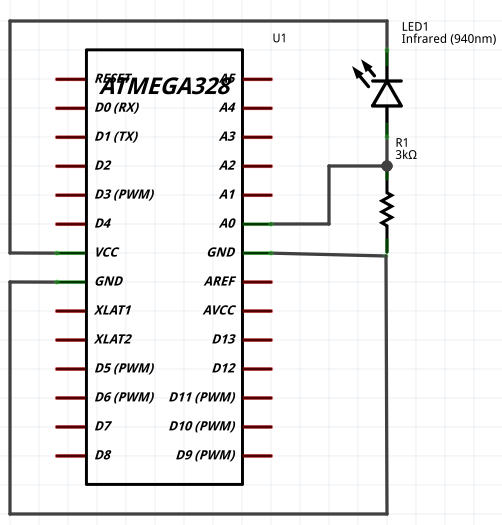
\includegraphics[width=4cm, height=3cm]{img/senlaesq.png} & 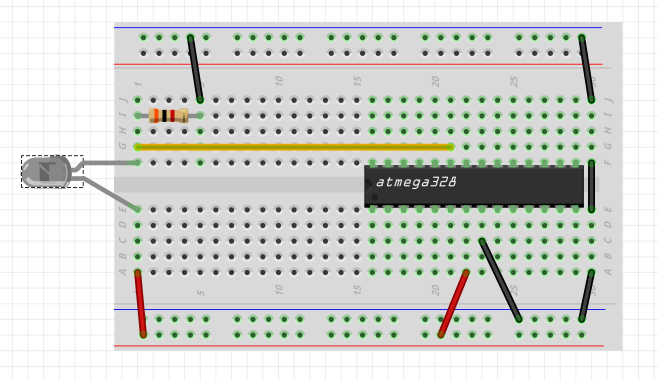
\includegraphics[width=4cm, height=3cm]{img/senlapro.png} \\ \hline
7.A. & 7.B. \\ \hline
\end{tabular}
\captionof{figure}{Figura 7.A Montaje eléctrico del sensor lateral infrarrojo conectado a tarjeta atmega 328 P-PU, con una resistencia de $3 k\Omega$. Figura 7.B Montaje en protoboard, los cables negros son tierra, los cables rojos son voltaje, y los cables naranjas son conexiones.}
\label{fig:g7}
\end{Figure}
Este sensor tiene la valiosa tarea de capturar datos del experimento que ilustrara el portento físico de la difracción en el espectro electromagnético infrarrojo. Por esta razón se destino su ubicación en el lado derecho del vehículo motorizado infrarossi como se observa en el anexo B-5.
\subsubsection{Sensor frontal emisor - receptor}
Las conexiones del sensor receptor frontal, se aprecia en la figura 8.A. y en la figura 8.B; conectar una resistencia de $3 k\Omega$ al ánodo del led receptor y el otro extremo de la resistencia a tierra, luego unir el pin 28 \footnote{Este pin es la entrada analógica numero cinco del microcontrolador atmega.} del microcontrolador en un punto intermedio entre la resistencia y el ánodo del diodo led receptor, el cátodo del diodo receptor se conecta a +5V.\\\\
Para la  fuente emisora de fotones infrarrojos o radiación infrarroja, se utiliza un diodo led emisor infrarrojo, el cátodo del diodo se une  a la resistencia de $500 \Omega$ y el otro extremo de la resistencia a tierra, el ánodo del diodo se conecta al pin 12\footnote{Salida D6 PWM.} del microcontrolador.\\
\begin{Figure}
\center
\begin{tabular}{|l|r|}
\hline
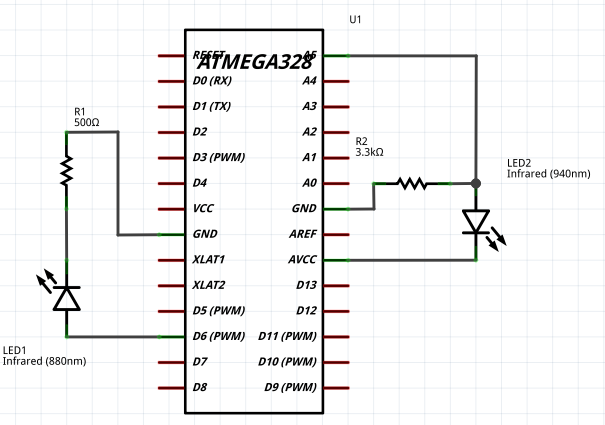
\includegraphics[width=4cm, height=4cm]{img/ledesq.png} & 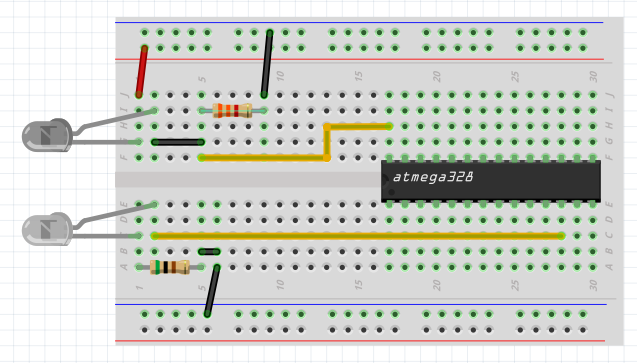
\includegraphics[width=4cm, height=4cm]{img/ledmont.png} \\ \hline
8.A & 8.B \\ \hline
\end{tabular}
\captionof{figure}{Figura 8.A Conexiones de los diodos receptor y emisor con microcontrolador atmega328P-PU. Figura 8.B Montaje en protoboard del sistema emisor receptor infrarrojo, junto a dos resistencias, y el microcontrolador, los cables negros son tierra, los cables rojos son voltaje, el cable naranja son conexiones.}
\label{fig:g8}
\end{Figure}
Estos dos dispositivos eléctricos colocados en la parte frontal del vehículo tienen la preciada tarea de ilustrar dos portentos físicos como lo son la atenuación de la irradiansa con el inverso del  cuadrado y la absorción debida a la interacción de la radiación electromagnética con la materia.
\subsubsection{Diodo led RGB}
Se utilizan tres diodos led de distintos colores o un diodo led rgb, con el fin de identificar el proceso que esta realizando el microcontrolador y sus diferentes sensores a través del titileo de los led's.
Las conexiones se aprecian en los esquemas de la figura 9.A y 9.B;  el ánodo del diodo rgb se conecta a +5V, el pin rojo del diodo rgb se conecta a una resistencia de $500\Omega$ y el otro extremo de la resistencia se conecta al pin 18 del microcontrolador, el pin verde del diodo rgb unido a una resistencia de $500\Omega$ y el otro extremo de la resistencia se conecta al pin 16 del microcontrolador, el pin azul del diodo se une a una resistencia de $500\Omega$ y el otro extremo de la resistencia se conecta al pin 15 del microcontrolador.\\
\begin{Figure}	
\center
\begin{tabular}{|l|r|}
\hline
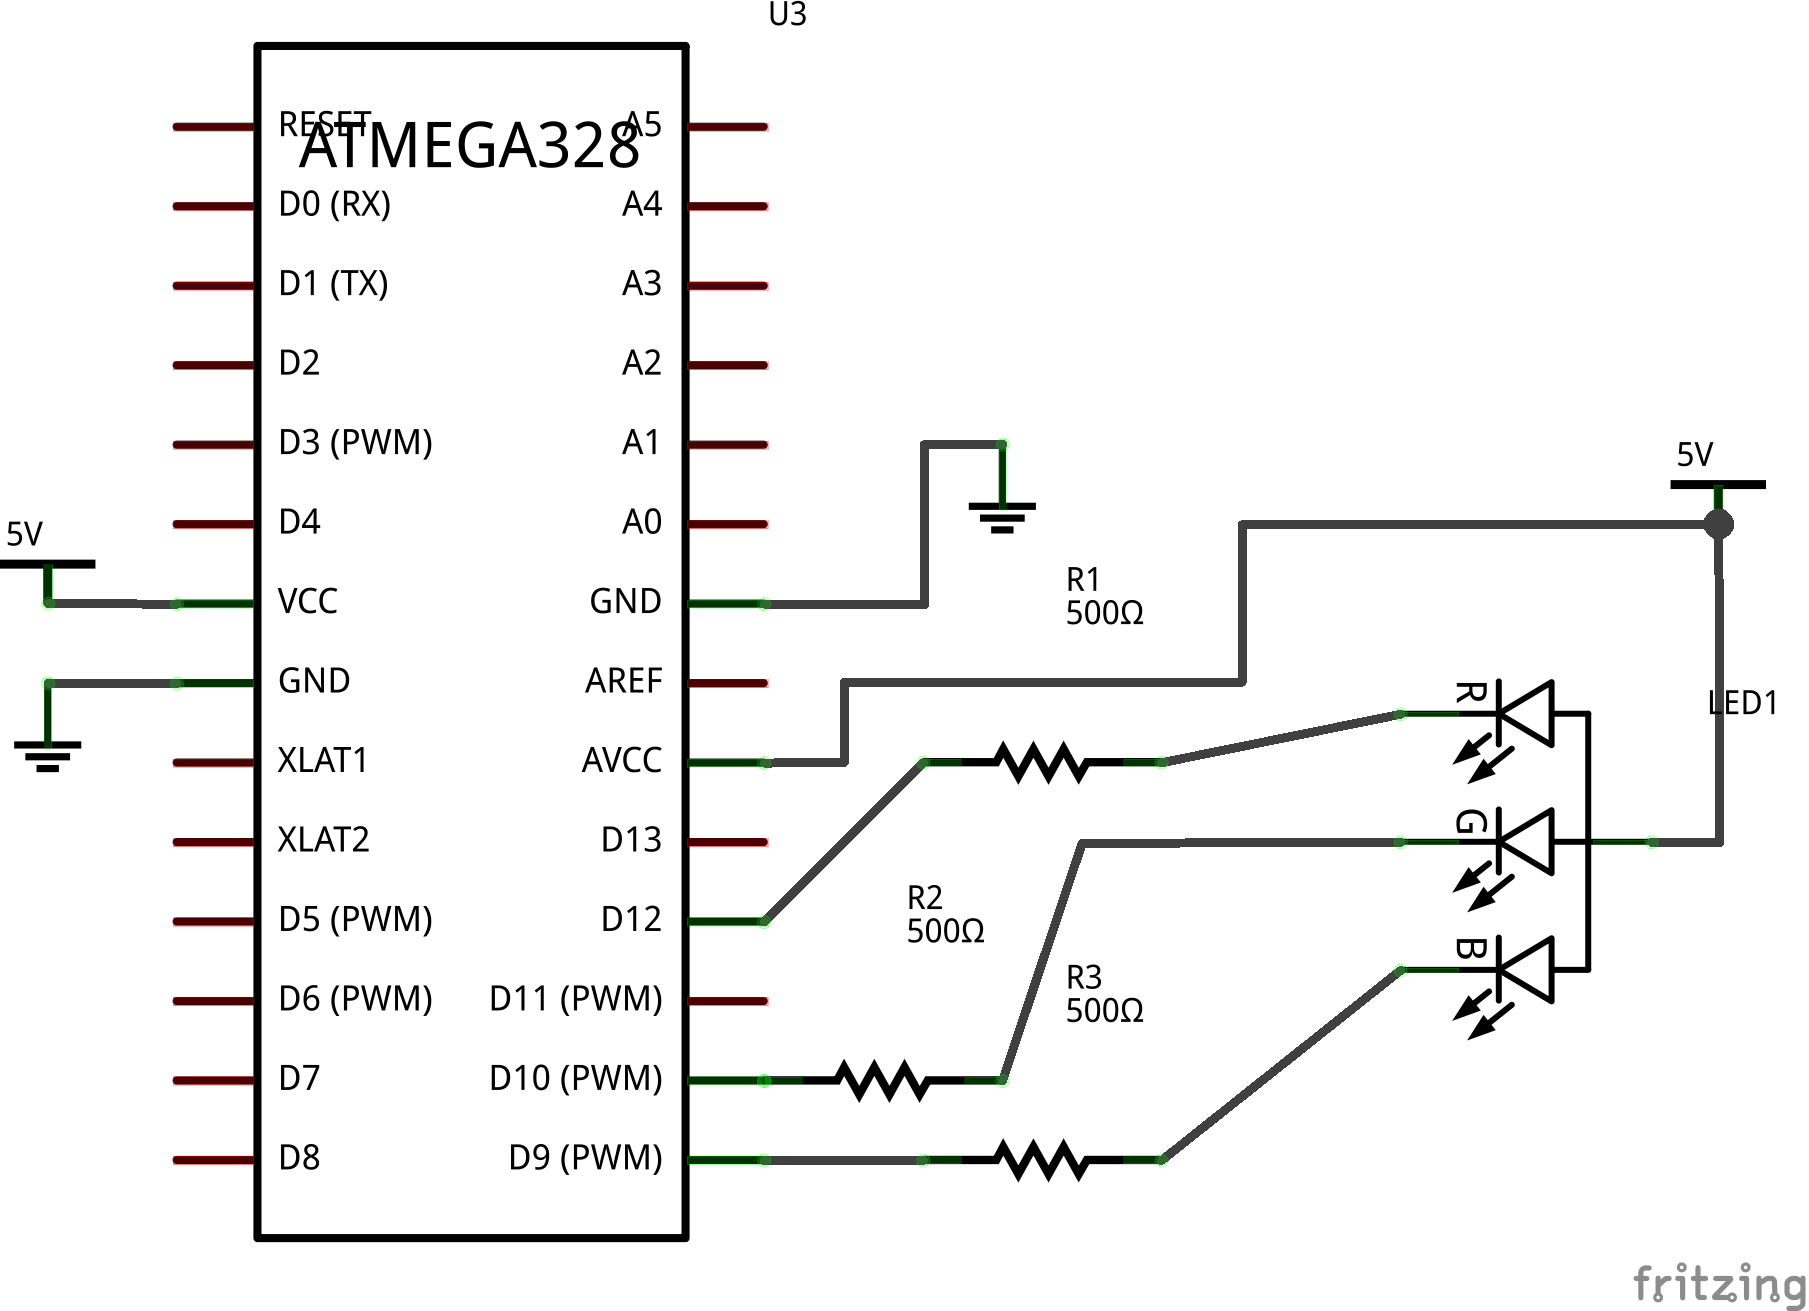
\includegraphics[width=4cm, height=3cm]{img/rgbesq.png} & 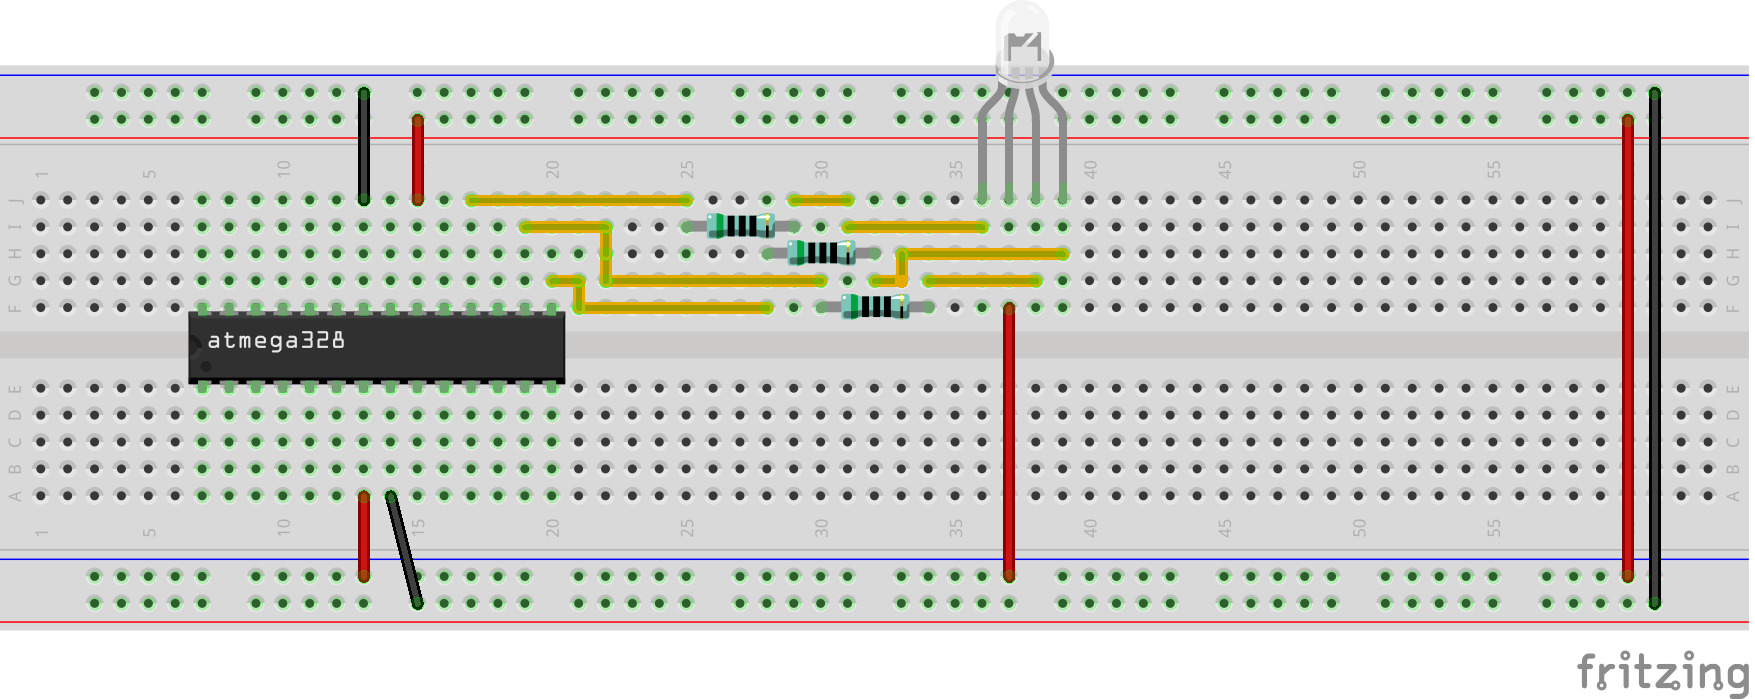
\includegraphics[width=4cm, height=3cm]{img/rgbmont.png} \\ \hline
9.A & 9.B \\ \hline
\end{tabular}
\captionof{figure}{Figura 9.A Circuito eléctrico diodo rgb con el microcontrolador atmega 328 P-PU. Figura 9.B Esquema  del diodo rgb en protoboard.}
\label{fig:g9}
\end{Figure}
El microcontrolador atmega 328P-Pu debe quedar en una sola tarjeta junto con el transformador de voltaje, el modulo bluetooth, el botón de reinicio, el oscilador y un enchufe para la batería de 9 voltios cuadrada como se muestra en la figura 10.
\begin{Figure}
\center
\begin{tabular}{|l|r|}
\hline
\\
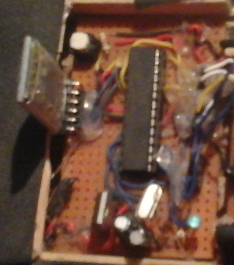
\includegraphics[width=4cm, height=5cm]{img/tar_tras.png}  \\\\ \hline
\end{tabular}
\captionof{figure}{Tarjeta electrónica con integrado atmega 328P-PU, oscilador 16 mHz, botón reinicio y bluetooth.}
\label{fig:g10}
\end{Figure}
Se coloca una cinta de color negro en los encapsulados epoxy de los sensores infrarrojos, esto con el fin de disminuir el ruido debido a fuentes externas de radiación infrarroja como se aprecia en la figura 11, el diodo emisor infrarrojo se deja sin cinta; ahora deben quedar estos sensores infrarrojos, el emisor infrarrojo y el regulador de rapidez del motor en una sola placa electrónica junto con el diodo RGB o diodos led de colores, asegurándose de dejar conexiones a la otra tarjeta con cables, pero sin unirlos hasta el montaje mecánico. 
\begin{Figure}
\center
\begin{tabular}{|l|r|}
\hline
\\
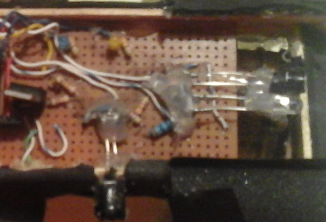
\includegraphics[width=6cm, height=4cm]{img/tar_frontal.png}  \\\\ \hline
\end{tabular}
\captionof{figure}{Tarjeta electrónica con sensores infrarrojos y emisor infrarrojo, junto con el control de rapidez del vehículo.}
\label{fig:g11}
\end{Figure}
%---------------aca empieza el montaje mecanico------------------
\subsection{Montaje mecánico}
Se debe cortar la tabla o acrílico con las medidas que se muestran en el anexo B.1; la placa electrónica de la figura 10 se ajusta en la parte trasera del vehículo y la placa de la figura 11 se une a la parte delantera del vehículo, después de esto se realizan las conexiones de las dos placas, tal como se observa en la figura 12.
\begin{Figure}
\center
\begin{tabular}{|l|r|}
\hline
\\
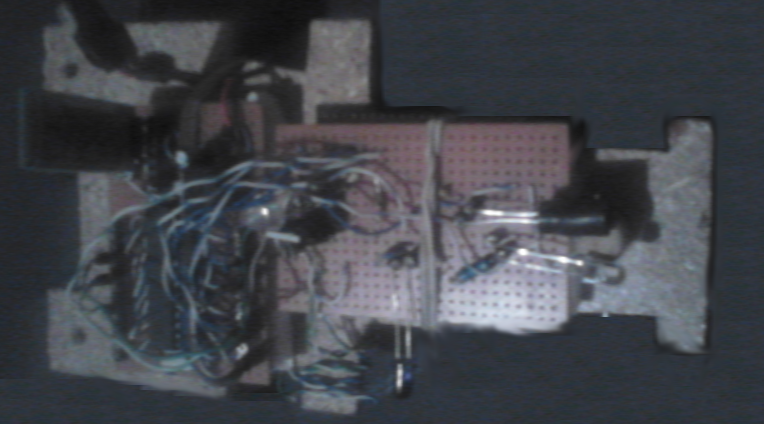
\includegraphics[width=8cm, height=5cm]{img/tar_com.png}  \\\\ \hline
\end{tabular}
\captionof{figure}{Placas electrónicas ajustadas al diseño final del chasis de madera.}
\label{fig:g12}
\end{Figure}
Para terminar el montaje mecánico se coloca el dispositivo de tracción electromagnética, por la parte contraria de donde se encuentran las tarjetas electrónicas del chasis junto con las llantas, como se muestra en los anexos B.2 y B.4. 
%------------------aca comienza la instalación del software----------------------------------------
\section{Software de control free infrarossi}
\subsection{¿Qué es free infrarossi?}
Free infrarossi es un  programa creado en Colombia, en la ciudad de Bogotá; el cual fue desarrollado con software libre y en un entorno libre como lo es GNU-Linux, no es multiplataforma, fue diseñado únicamente para este sistema operativo; se vale de lenguajes de programación, como  C, C++, python 2.7, bash; y de programas como arduino, octave, gnuplot, blueman-manager entre otros, fusionados en una interfaz amigable y fácil de utilizar. \\\\
Free infrarossi es un instrumento de laboratorio que ilustra  la propiedad de difracción, atenuación y absorción de ondas electromagnéticas en el espectro infrarrojo, esta diseñado para ser utilizado tanto por  estudiantes como docentes de muy diversas ramas de las ciencias y  la ingeniería o como una herramienta muy útil para los educadores y alumnos de media vocacional.
\subsection{Licencia}
Programa de control de hardware e ilustración física de las propiedades de las ondas electromagnéticas en el espectro infrarrojo.\\\\
Copyright (C) 2016-01-01  Universidad Distrital Francisco Jose, Diego Alberto Parra Garzón, Dr. Julian Andres Salamanca Bernal. \\\\
El programa free infrarossi es software libre; puedes redistribuirlo y / o modificarlo bajo los términos de la Licencia Pública General GNU publicada por la Fundación para el Software Libre; ya sea 	la versión 3 de la Licencia, o (a su elección) cualquier versión posterior. \\\\
Este programa se distribuye con la esperanza de que sea útil, pero SIN NINGUNA GARANTÍA; ni siquiera la garantía implícita de COMERCIALIZACIÓN o IDONEIDAD PARA UN PROPÓSITO PARTICULAR. Vea la Licencia Pública General GNU para más detalles. \\\\
Debería haber recibido una copia de la Licencia Pública General de GNU junto con este programa; si no, escriba a la Free Software Foundation, Inc., 51 Franklin Street, Quinto Piso, Boston, MA 02110-1301 EE.UU..\\\\
Si usted hace alguna modificación en esta aplicación, deberá siempre mencionar el autor original de la misma.
\subsection{Instalación}
La instalación de este software es relativamente sencilla, el proceso de instalación es el mismo para distribuciones basadas en Debian\footnote{Pagina oficial proyecto Debian https://www.debian.org/} se  explicara paso a paso el proceso de instalación:
\begin{enumerate}
\item[a.] Abrir una terminal\footnote{Enlace que explica ese procedimiento: http://www.comoinstalarlinux.com/como-abrir-una-terminal-en-ubuntu-linux-mint-centos-debian/} y escribir en ella lo siguiente sin comillas $"$sudo su$"$ y luego oprimir la tecla enter.
\item[b.] Escribir la contraseña de administrador y presione enter; tenga en cuenta que la terminal no muestra la contraseña.
\item[c.] Escriba en la terminal sin comillas $"$aptitude install -y git$"$, presione enter.
\item[d.] Escriba en la terminal sin comillas $"$cd Documentos$"$ presione enter.
\item[e.] Escriba en la terminal sin comillas $"$git clone https://github.com/Diego-debian/Free-infrarossi$"$, presione enter.
\item[f.] Escriba en la terminal sin comillas $”$chmod +777 Free-infrarossi$”$, presione la tecla enter.
\item[g.] Cierre la terminal y diríjase al navegador de archivos o gestor de archivos y ábralo.
\item[h.] Diríjase a la carpeta Documentos/Free-infrarossi/\\install.
\item[j.] Hacer click derecho con el mouse en el archivo instalador.py,  dar click izquierdo en propiedades; en la pestaña de general debe decir abrir archivo con python 2.7 y en la pestaña permisos debe estar seleccionada la casilla permitir ejecutar este archivo como programa, de no ser así cambie las opciones y déjelas como se menciono antes.
\item[k.] Cierre la ventana y abra el archivo INSTALADOR.py haciendo doble click izquierdo sobre este.
\item[l.] Escriba su contraseña de administrador y presione enter.
\item[m.] Una vez abierto el instalador escriba  1 y presione enter.
\item[n.] Escriba nuevamente 1 y enter.
\item[ñ.] Una vez finalizada la instalación se aconseja reinicie su pc.
\end{enumerate}
\subsection{Primer uso free infrarossi}
Una vez este reiniciado el computador, lo primero  es abrir una terminal del S.O. escribir en la terminal sin comillas $'infrarossi'$ y oprimir la tecla enter, escribir la clave de administrador y se abrirá la ventana del software free infrarossi, como se aprecia en la figura 13.
\begin{Figure}	
\center
\begin{tabular}{|l|r|}
\hline \\
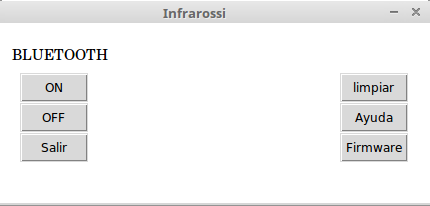
\includegraphics[width=8cm, height=3cm]{img/infrarossi.png} \\ \hline
%10. \\ \hline 
\end{tabular}
\captionof{figure}{Ventana del software free infrarossi}
\label{fig:g13}
\end{Figure}
\subsection{Carga de firmware en integrado atmega 328 P-PU}
En la ventana del programa free infrarossi, en la parte inferior derecha hay tres botones, oprimir el botón de firmware y conectar la tarjeta micro controladora arduino uno al pc; acto seguido oprimir el botón continuar y esperar que cargue el firmware en la tarjeta, una vez hecho esto retirar el micro controlador de la tarjeta y colocarlo en el montaje del vehículo como se observa en la figura 14.
\begin{Figure}	
\center
\begin{tabular}{|l|r|}
\hline\\
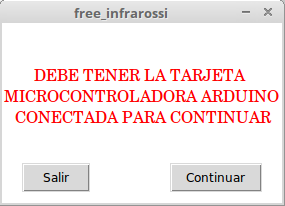
\includegraphics[width=8cm, height=4cm]{img/firmware.png} \\ \hline
%11. \\ \hline
\end{tabular}
\captionof{figure}{Ventana de instalación del firmware, que ofrece el software free infrarossi, para el vehículo motorizado infrarossi.}
\label{fig:g14}
\end{Figure}
%-----------uso avanzado del software de control----------------------------------
\subsection{Uso avanzado de free infrarossi}
Tanto el vehículo infrarossi y el software de control se diseñaron específicamente para ilustrar tres propiedades de la radiación electromagnética en el espectro infrarrojo, por esta razón el software cuenta con un botón de encendido o por su nombre en ingles $on$, al hacer click sobre este, el programa envía la solicitud de emparejamiento al vehículo motorizado infrarossi, una vez hecho el protocolo de reconocimiento y de emparejarse ambos dispositivos; se despliega un tercer menú en la ventana del software como se muestra en la figura 15.
\begin{Figure}	
\center
\begin{tabular}{|l|r|}
\hline\\
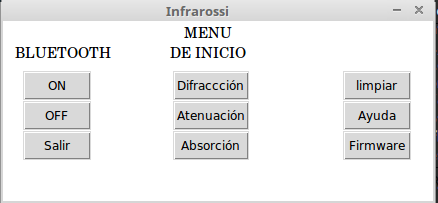
\includegraphics[width=8cm, height=3cm]{img/3menu.png} \\ \hline
%11. \\ \hline
\end{tabular}
\captionof{figure}{Ventana del software de control free infrarossi, con  bluetooth encendido y el menú para los portentos físicos.}
\label{fig:g15}
\end{Figure}
Es importante aclarar que el firmware del modulo motorizado free infrarrossi esta diseñado para ordenar un voltaje de $3 V$ al motor desde el microcontrolador, de esta manera circula una corriente de $12 mA$ durante un tiempo de 37 $ms$ por el embobinado del motor, obteniendo un avance de  $2 mm$ con un margen de error del $9\%$; después de esto el motor no recibe más corriente por lo que se detiene y el microcontrolador le ordena a los sensores infrarrojos que  comiencen su trabajo, según el montaje experimental que se este realizando.
%--------------------boton difraccion---------------------------------------
\subsubsection{Botón difracción}
El montaje experimental para la demostración del fenómeno de difracción en el espectro infrarrojo se encuentra explicado en el anexo C.1; una vez esta listo el montaje de laboratorio para la captura de datos del portento de la difracción por el vehículo motorizado free infrarossi, oprimir el botón difracción en la ventana del software de control,  inmediatamente el software de control empezara a capturar los datos del experimento y los almacena en el ordenador para su respectivo análisis, este proceso se muestra en la figura 16.
\begin{Figure}	
\center
\begin{tabular}{|l|r|}
\hline\\
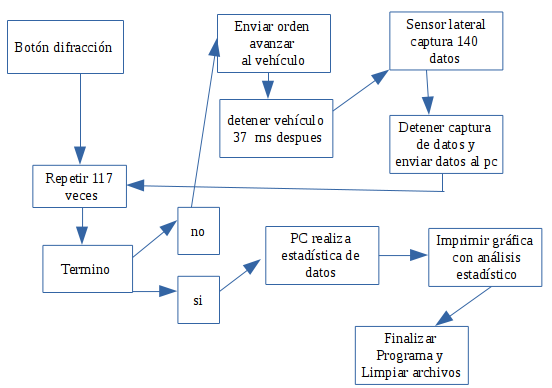
\includegraphics[width=8cm, height=5cm]{img/diagrama1.png} \\ \hline
%11. \\ \hline
\end{tabular}
\captionof{figure}{Diagrama de control del software y hardware en el experimento de difracción.}
\label{fig:g16}
\end{Figure}
Una vez terminado el proceso de captura y análisis de datos el software de control llama a la librería matplotlib de python 2.7 para crear la gráfica de los datos con su respectivo análisis y el error en las medidas del laboratorio.
%--------------------boton atenuacion---------------------------------------
\subsubsection{Botón atenuación}
El montaje experimental para la demostración del fenómeno de atenuación en el espectro infrarrojo se encuentra explicado en el anexo C.2; una vez esta listo el montaje de laboratorio para la captura de datos del fenómeno de la atenuación por el vehículo motorizado free infrarossi, oprimir el botón atenuación en la ventana del software de control,  inmediatamente el software de control empezara a capturar los datos del experimento y los almacena en el ordenador para su respectivo análisis, este proceso se muestra en la figura 17.
\begin{Figure}	
\center
\begin{tabular}{|l|r|}
\hline\\
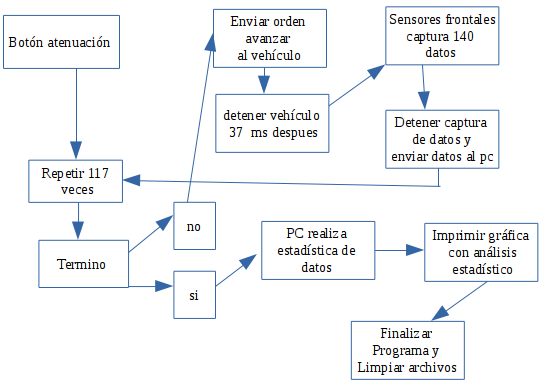
\includegraphics[width=8cm, height=5cm]{img/diagrama2.png} \\ \hline
%11. \\ \hline
\end{tabular}
\captionof{figure}{Diagrama de control del software y hardware en el experimento de atenuación.}
\label{fig:g17}
\end{Figure}
Una vez terminado el proceso de captura y análisis de datos el software de control llama a la librería matplotlib de python 2.7 para crear la gráfica de los datos con su respectivo análisis y el error en las medidas del laboratorio.
%--------------------boton absorción ---------------------------------------
\subsubsection{Botón absorción}
El montaje experimental para la demostración del fenómeno de absorción en el espectro infrarrojo se encuentra explicado en el anexo C.3; una vez esta listo el montaje de laboratorio para la captura de datos del fenómeno de la absorción por el vehículo motorizado free infrarossi, oprimir el botón absorción en la ventana del software de control,  inmediatamente el software de control empezara a capturar los datos del experimento y los almacena en el ordenador para su respectivo análisis, este proceso se muestra en la figura 18.
\begin{Figure}	
\center
\begin{tabular}{|l|r|}
\hline\\
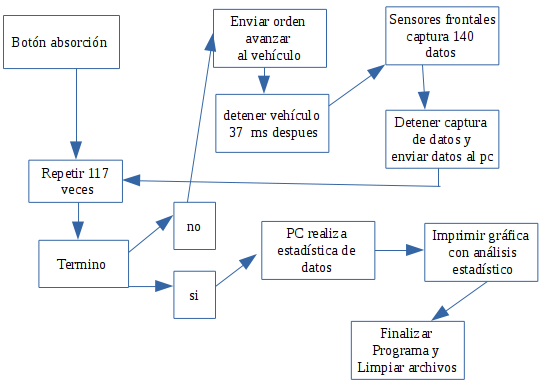
\includegraphics[width=8cm, height=5cm]{img/diagrama3.png} \\ \hline
%11. \\ \hline
\end{tabular}
\captionof{figure}{Diagrama de control del software y hardware en el experimento de absorción.}
\label{fig:g17}
\end{Figure}
Una vez terminado el proceso de captura y análisis de datos el software de control llama a la librería matplotlib de python 2.7 para crear la gráfica de los datos con su respectivo análisis y el error en las medidas del laboratorio.
\section{Conclusiones}
\begin{enumerate}
\item[*] Las tecnologías libres favorecen la enseñanza y aprendizaje de las ciencias.
\item[*] Con la ayuda del software y hardware libre, se construyo el diseño de un vehículo motorizado  y su respectivo software de control, el cual es económico, preciso y capaz de demostrar tres portentos físicos de la física de las ondas electromagnéticas.
\item[*] La física que se encuentra de manera implícita y explicita en este trabajo hace que el instrumento motorizado infrarossi y su software de control free infrarossi sea un herramienta indispensable  en el aula de clase, así por profesionales en las ramas de las ciencias, como de los educandos, también es un modelo didáctico pedagógico que contribuye a la enseñanza en ciencias de los estudiantes de media vocacional grado once de diferentes instituciones educativas. 
\item[*] Utilizar los fenómenos de transporte de energía para la comunicación vía bluetooth, es una característica del proyecto que favorece su tamaño y la movilidad tanto física - mecánica del vehículo motorizado, como el procesamiento de esta información por el ordenador, facilitando estos procesos de análisis en el experimento del investigador. 
\end{enumerate}
\begin{thebibliography}{99}
\bibitem{ARDUINO} Monk, S. (2013). 30 Arduino projects for the evil genius. McGraw-Hill Professional.
\bibitem{REGULADOR} Semiconductor, F. (2012). LM7805 Data Sheet. [Online]. Disponible en:\\ http://pdf.datasheetcatalog.net/datasheet/fairchild/\\LM7805.pdf
\bibitem{TIP122} Semiconductor, F. (2008). Tip120/tip121/tip122 npn epitaxial darlington transistor. TIP120 datasheet, Oct. [Online]. Disponible en:\\ http://pdf.datasheetcatalog.net/datasheet/fairchild/\\TIP122.pdf.
% \bibitem{DIODO}  Hoja de datos diodo regulador 1N4001. http://pdf.datasheetcatalog.net/datasheet/lrc/\\1N4001.pdf
%\bibitem{INFRARED} Hoja de datos de los diodos led infrarrojos, emisor y receptor. \\ http://www.datasheetarchive.com/dlmain/Datasheets\\-31/DSA-617614.pdf
\bibitem{FRITZING} Knörig, A., Wettach, R., \& Cohen, J. (2009, February). Fritzing: a tool for advancing electronic prototyping for designers. In Proceedings of the 3rd International Conference on Tangible and Embedded Interaction. ACM.
\bibitem{PYTHON} Gift, N., \& Jones, J. M. (2008). Python for Unix and Linux system administration. ``O'Reilly Media, Inc.".
\bibitem{CIRCUITOS} Alexander, C. K., Sadiku, M. N., Bermúdez, A. V., \& Pedraza, C. R. C. (2006). Fundamentos de circuitos eléctricos. McGraw-Hill. 
\end{thebibliography}
\end{multicols}
%\clearpage % o \cleardoublepage
\selectlanguage{spanish}
\appendix
\addappheadtotoc
\appendixpage
\section{Esquemas}
\subsection{Montaje final protoboard}
\begin{Figure}	
\center
\fbox{
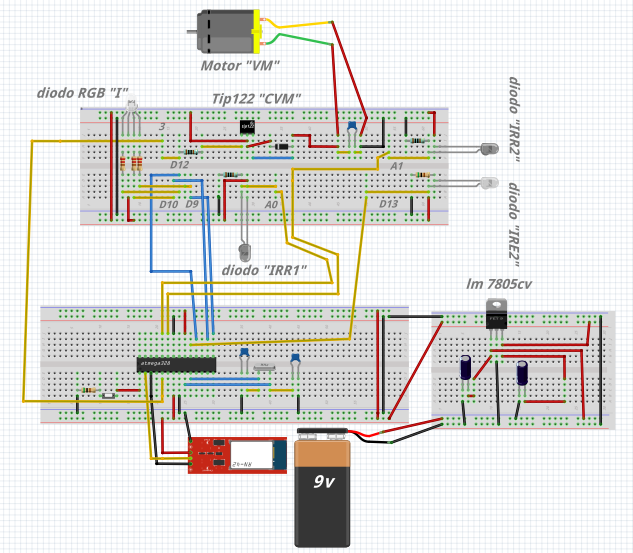
\includegraphics[width=18cm, height=15cm, angle=90]{img/montajep.png} 
	}
\captionof{figure}{Montaje eléctrico final.}
\label{fig:A}
\end{Figure}
%------------------------------------------------------------------------------
%---------------imagen---------------------------------------------------------
\subsection{Circuito eléctrico final.}
\begin{Figure}	
\center
\fbox{
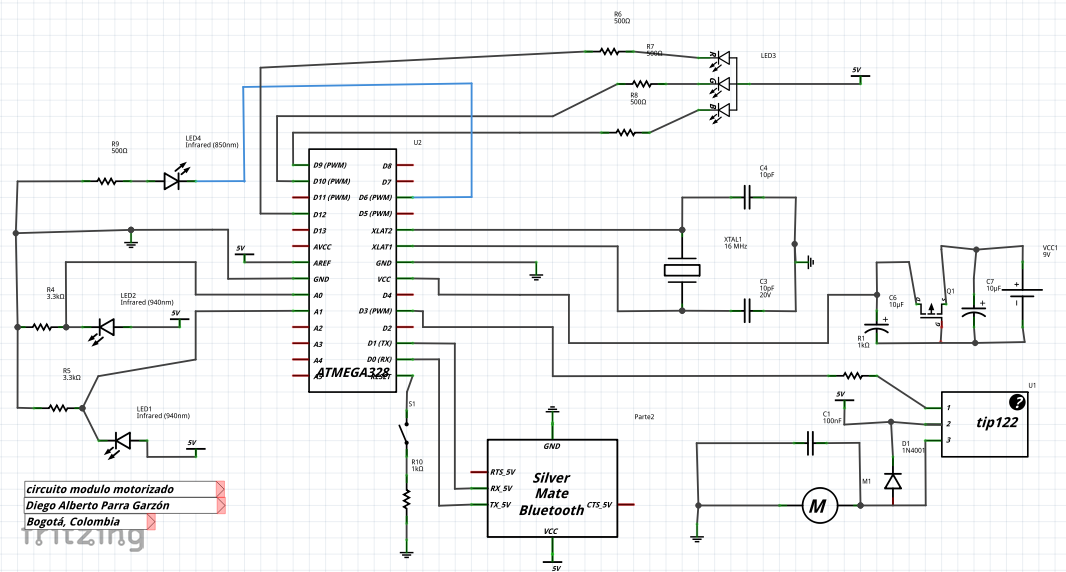
\includegraphics[width=19cm, height=15cm, angle=90]{img/esquemap.png} 
	}
\captionof{figure}{Circuito eléctrico del proyecto.}
\label{fig:B}
\end{Figure}
%------------------------------------------------------------------------------
%---------------imagen---------------------------------------------------------
\section{Chasis}
\subsection{Dimensiones del chasis}
\begin{Figure}	
\center
\fbox{
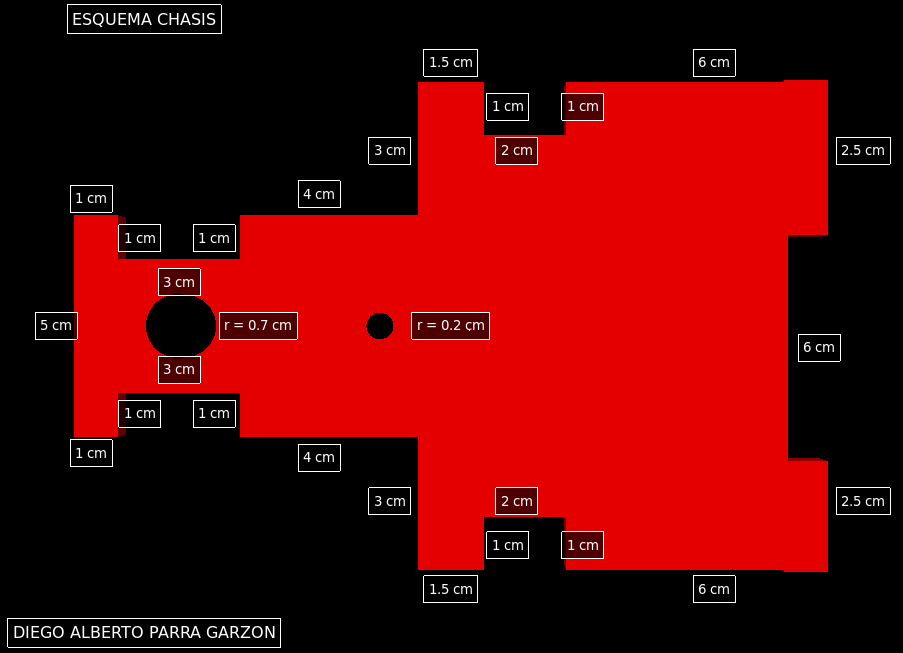
\includegraphics[width=18cm, height=15cm, angle=-90]{img/chasis.png} 
	}
\captionof{figure}{Dimensiones del chasis o base donde reposara el circuito eléctrico, el sistema de transmisión y demas elementos del vehiculo. Figura modelada en python visual.}
\label{fig:C}
\end{Figure}
%------------------------------------------------------------------------------
%---------------imagen---------------------------------------------------------
\subsection{Montaje simulado vista inferior}
\begin{Figure}	
\center
\fbox{
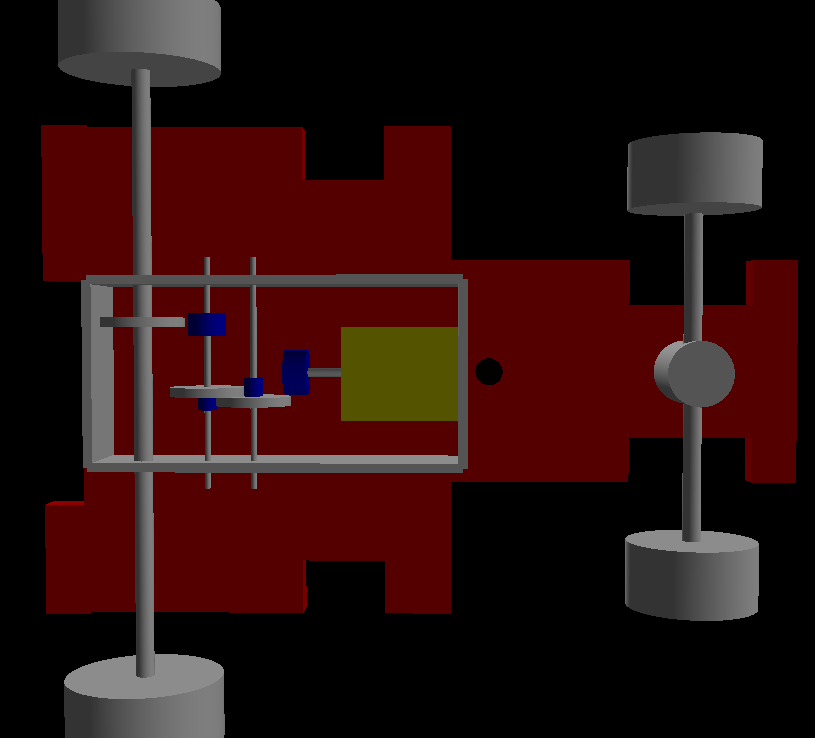
\includegraphics[width=9cm, height=7.5cm, angle=180]{img/montaje2.png} 
	}
\captionof{figure}{Vista inferior del montaje del vehículo con la transmisión y el eje delantero, sin la parte eléctrica. Figura modelada en python visual.}
\label{fig:D}
\end{Figure}
%------------------------------------------------------------------------------
%---------------imagen---------------------------------------------------------
\subsection{Montaje simulado vista superior}
\begin{Figure}	
\center
\fbox{
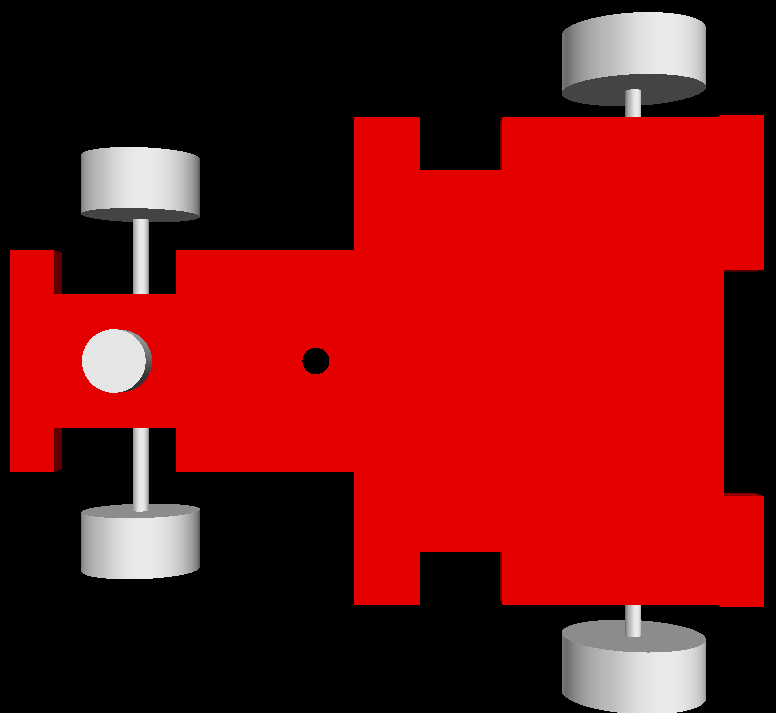
\includegraphics[width=9cm, height=7.5cm, angle=180]{img/montaje1.png} 
	}
\captionof{figure}{Vista superior del montaje del vehículo con la transmisión y el eje delantero, sin la parte eléctrica. Figura modelada en python visual.}
\label{fig:E}
\end{Figure}
%------------------------------------------------------------------------------
%---------------imagen---------------------------------------------------------
\subsection{Montaje real vista inferior}
\begin{Figure}	
\center
\fbox{
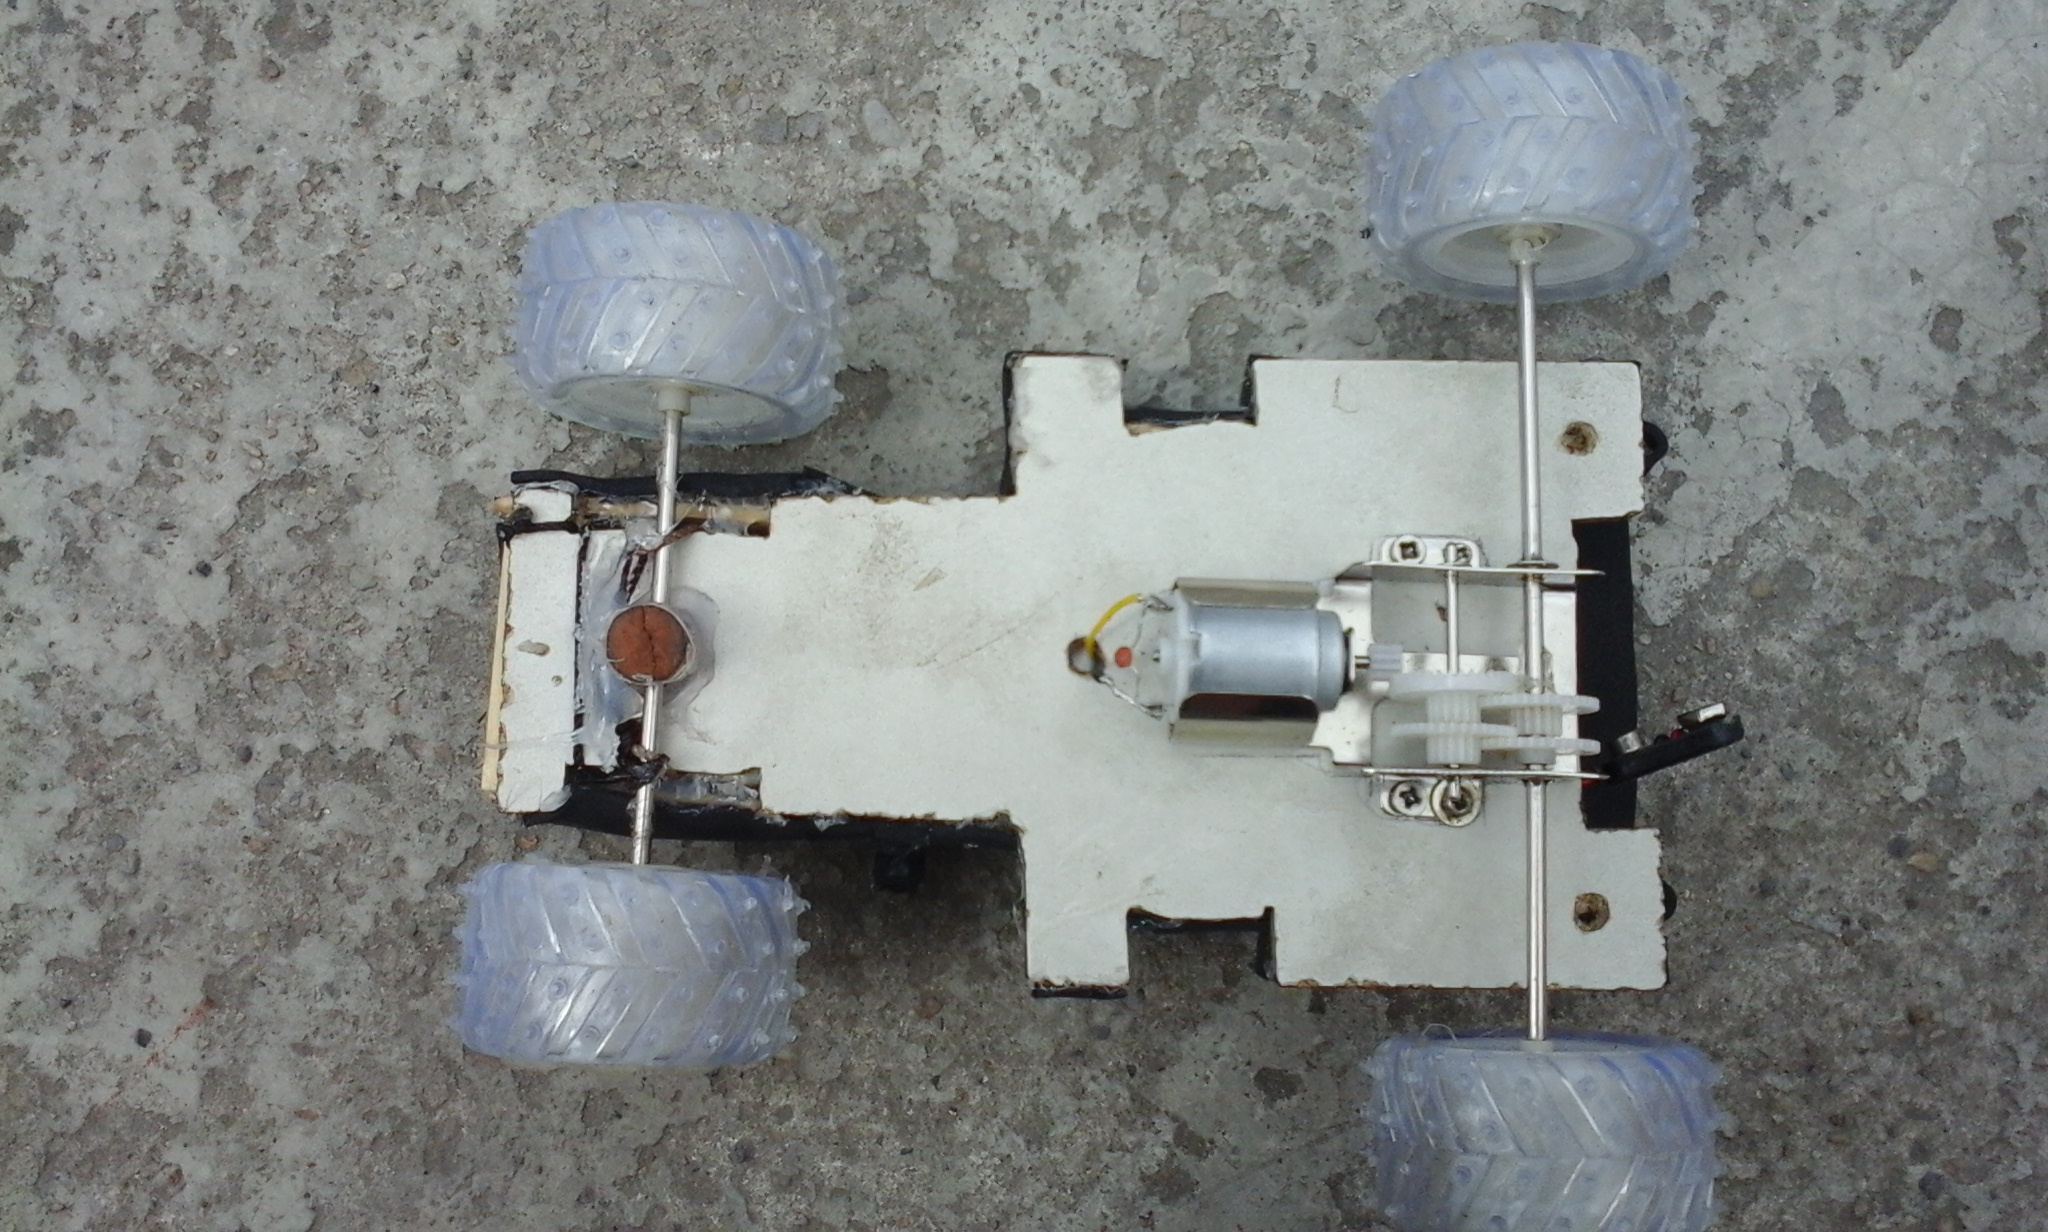
\includegraphics[width=12cm, height=7.5cm, angle=180]{img/monreal2.png} 
	}
\captionof{figure}{Vista inferior del montaje.}
\label{fig:F}
\end{Figure}
%------------------------------------------------------------------------------
%---------------imagen---------------------------------------------------------
\subsection{Montaje real vista superior}
\begin{Figure}	
\center
\fbox{
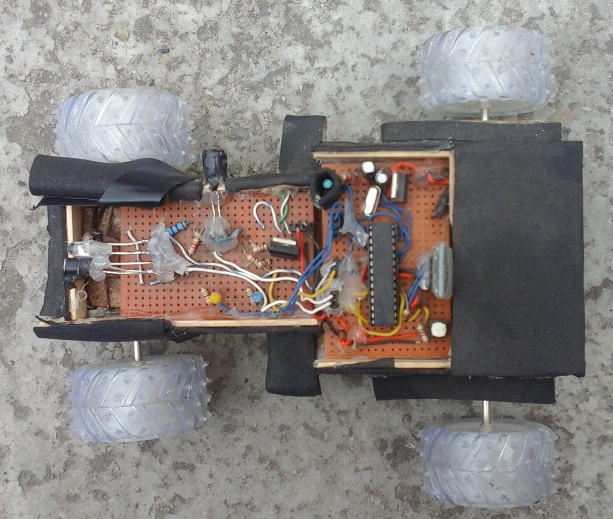
\includegraphics[width=12cm, height=8cm, angle=0]{img/monreal3.png} 
	}
\captionof{figure}{Vista superior del montaje.}
\label{fig:G}
\end{Figure}
\subsection{Montaje final}
\begin{Figure}	
\center
\fbox{
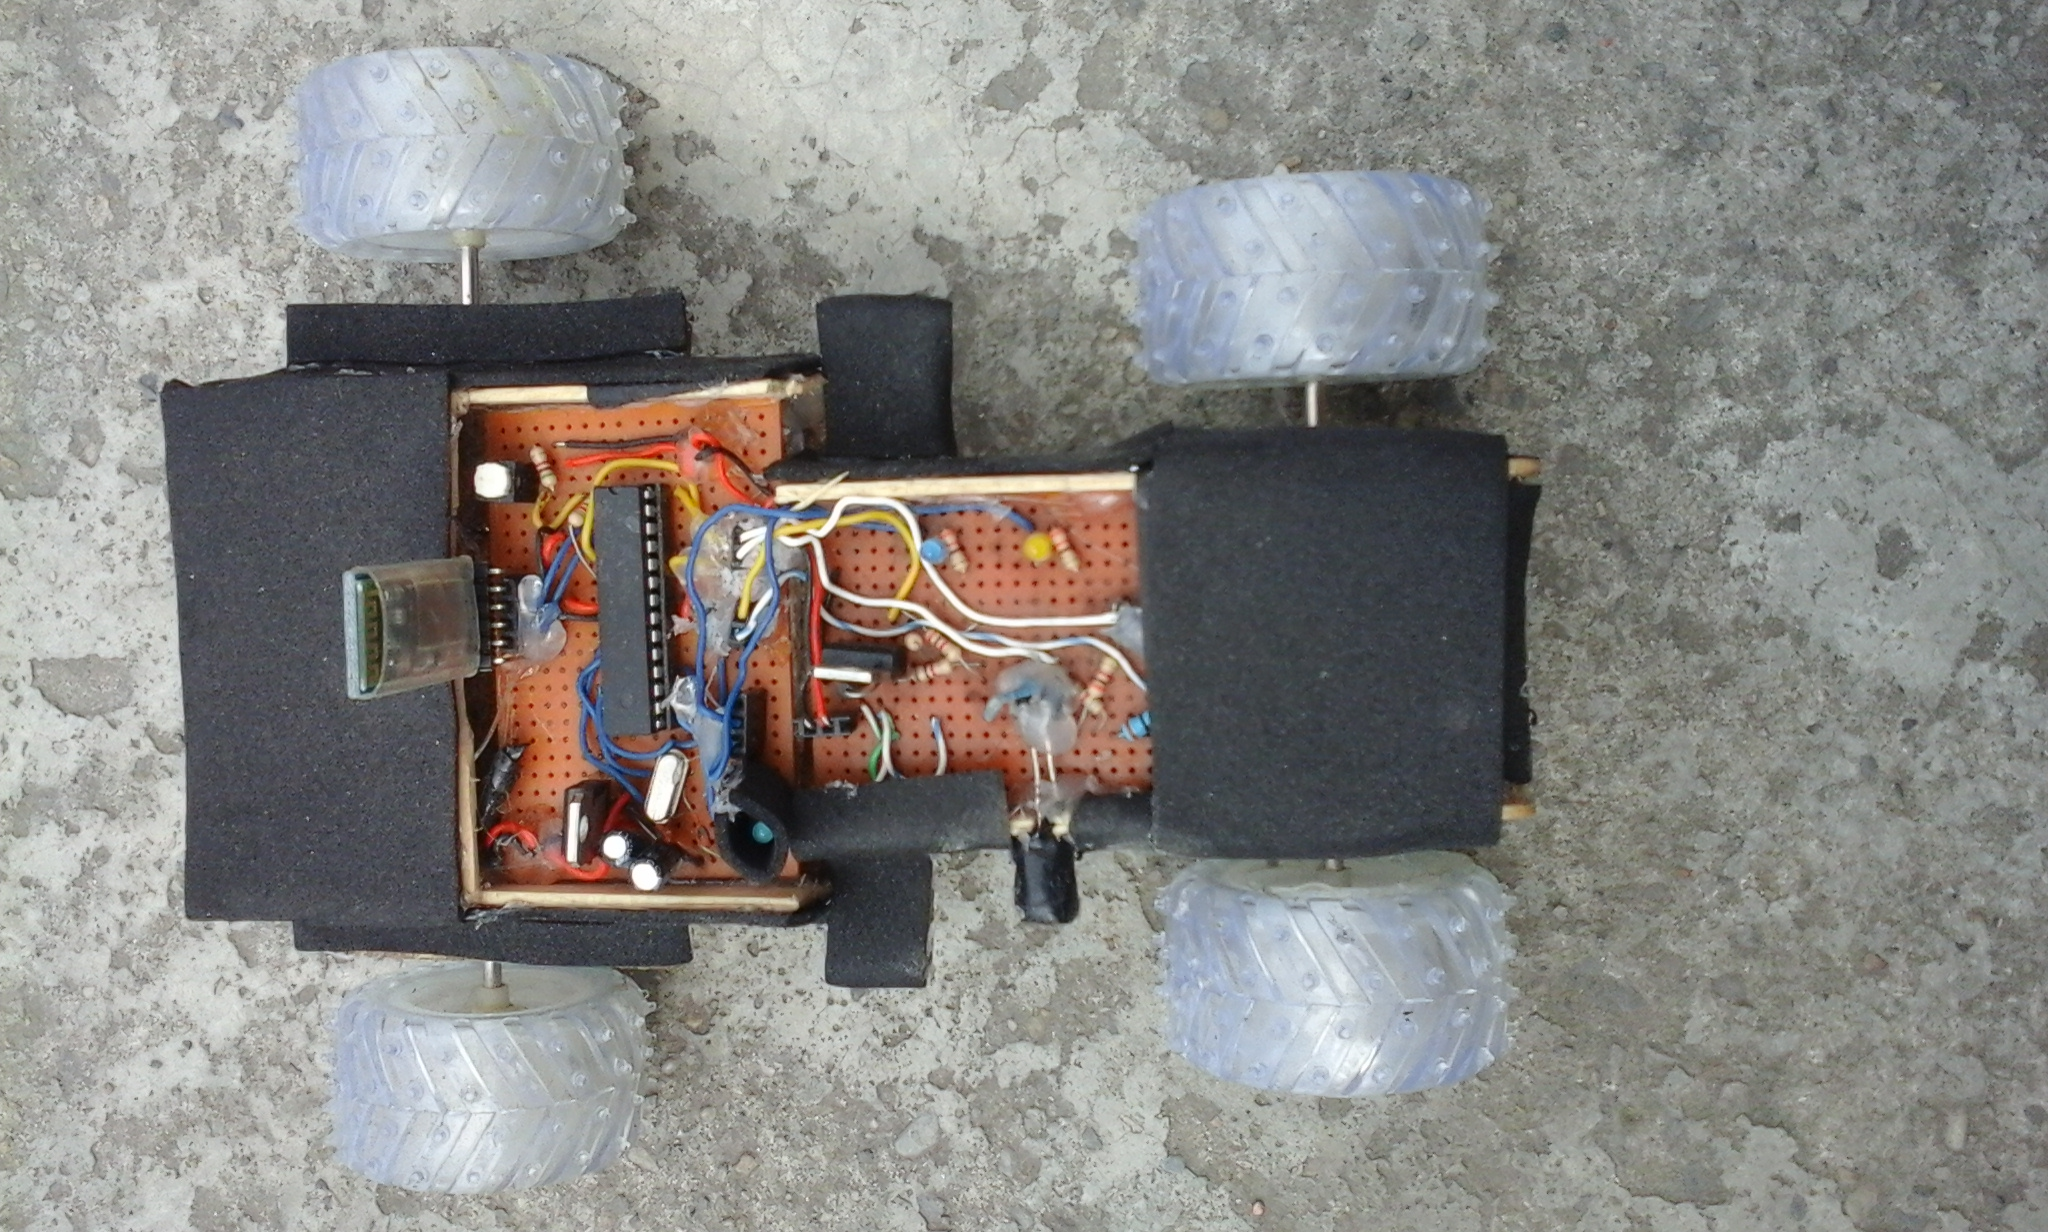
\includegraphics[width=14cm, height=9cm, angle=180]{img/monreal1.png} 
	}
\captionof{figure}{Vista superior del montaje.}
\label{fig:H}
\end{Figure}
%------------------------------------------------------------------------------
%\subsection{Montaje vista frontal}
%\begin{Figure}	
%\center
%\fbox{
%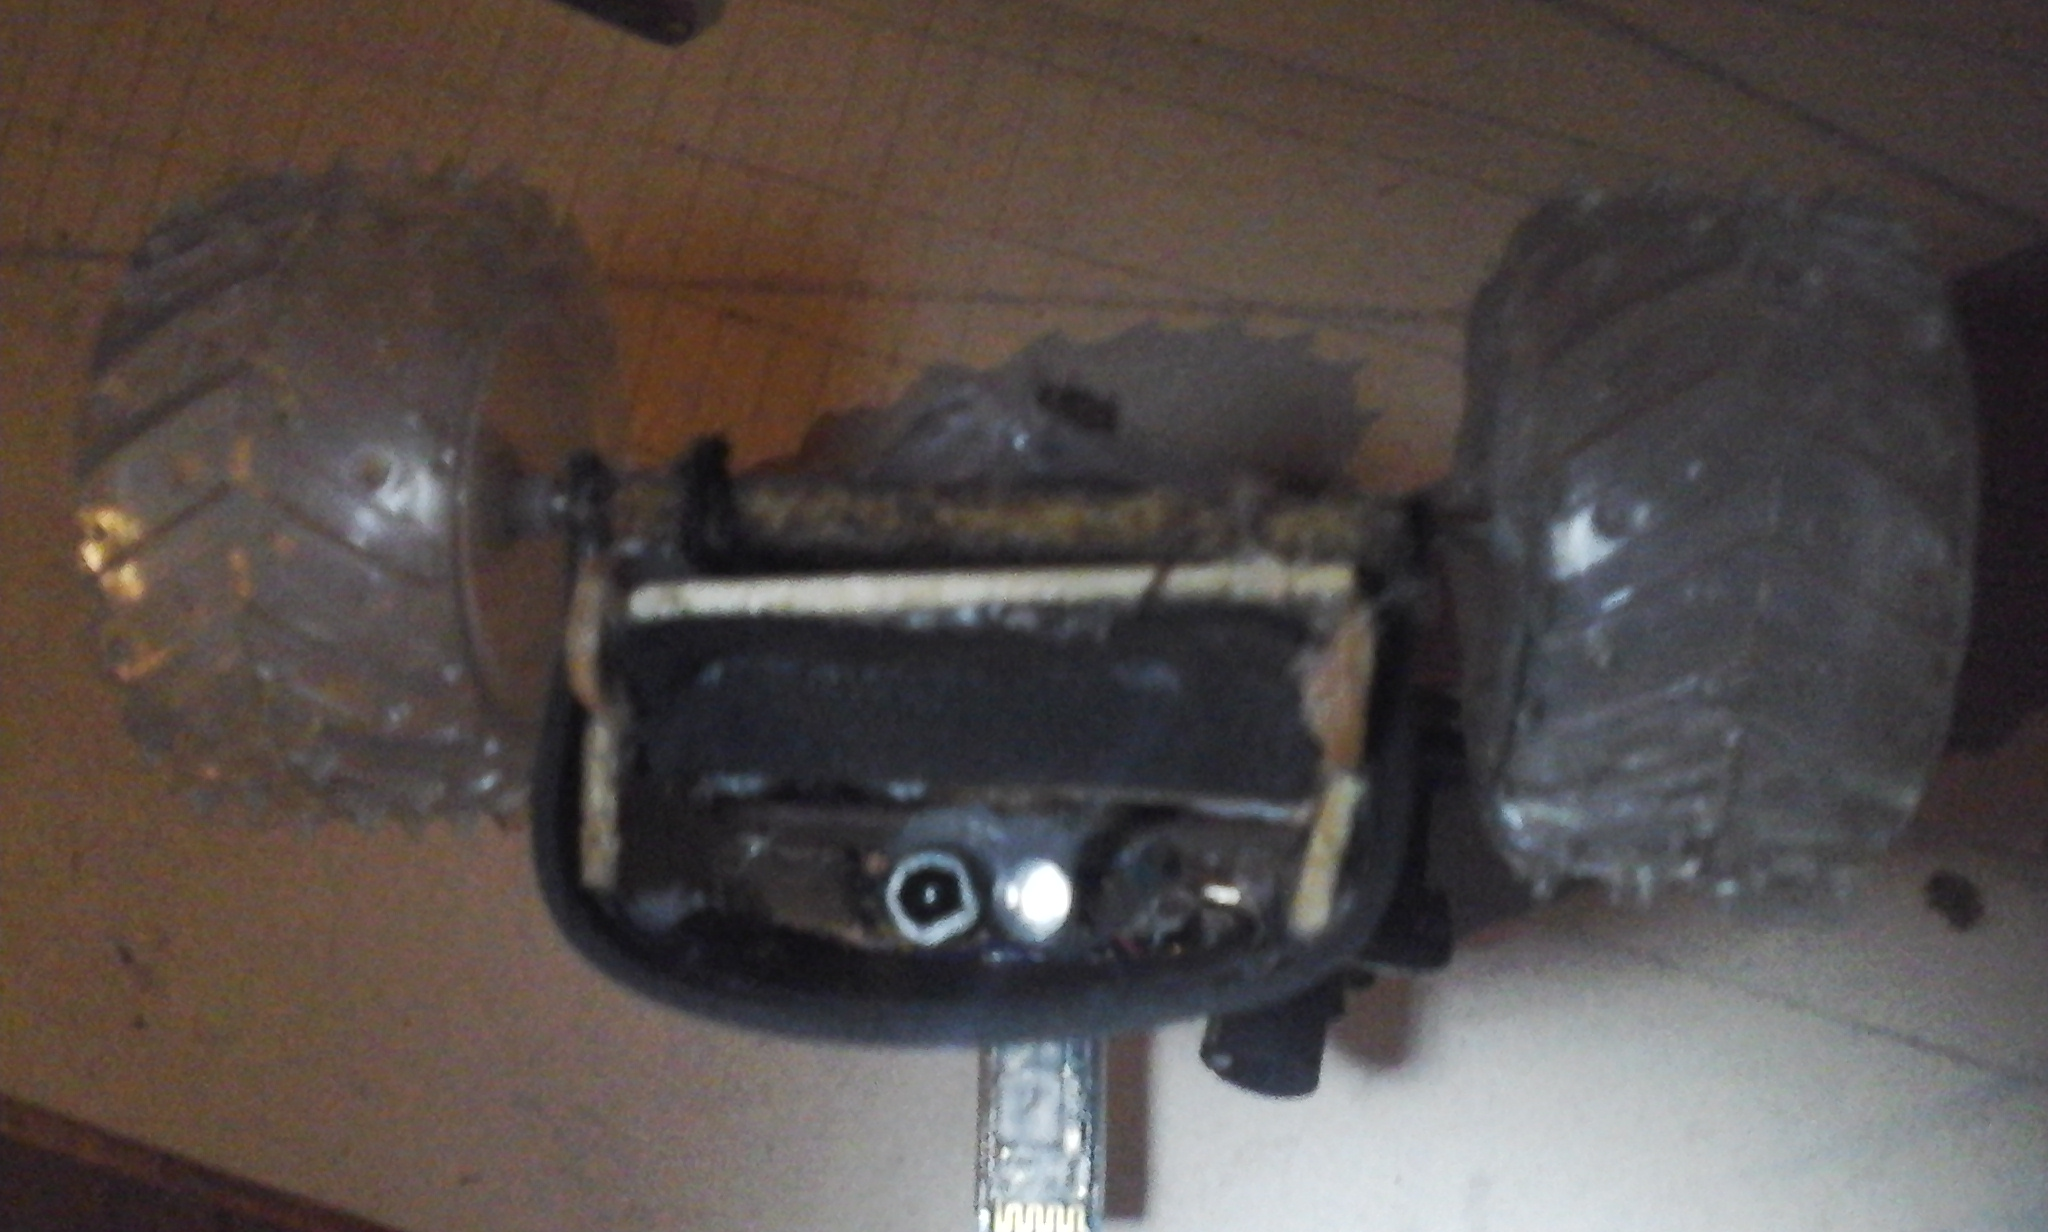
\includegraphics[width=12cm, height=7.5cm, angle=180]{img/vistafront.png} 
%	}
%\captionof{figure}{Vista frontal montaje.}
%\label{fig:H}
%\end{Figure}
\newpage
\section{Articulos}
\subsection{Articulo difracción}
Este articulo comienza en la pagina que sigue.
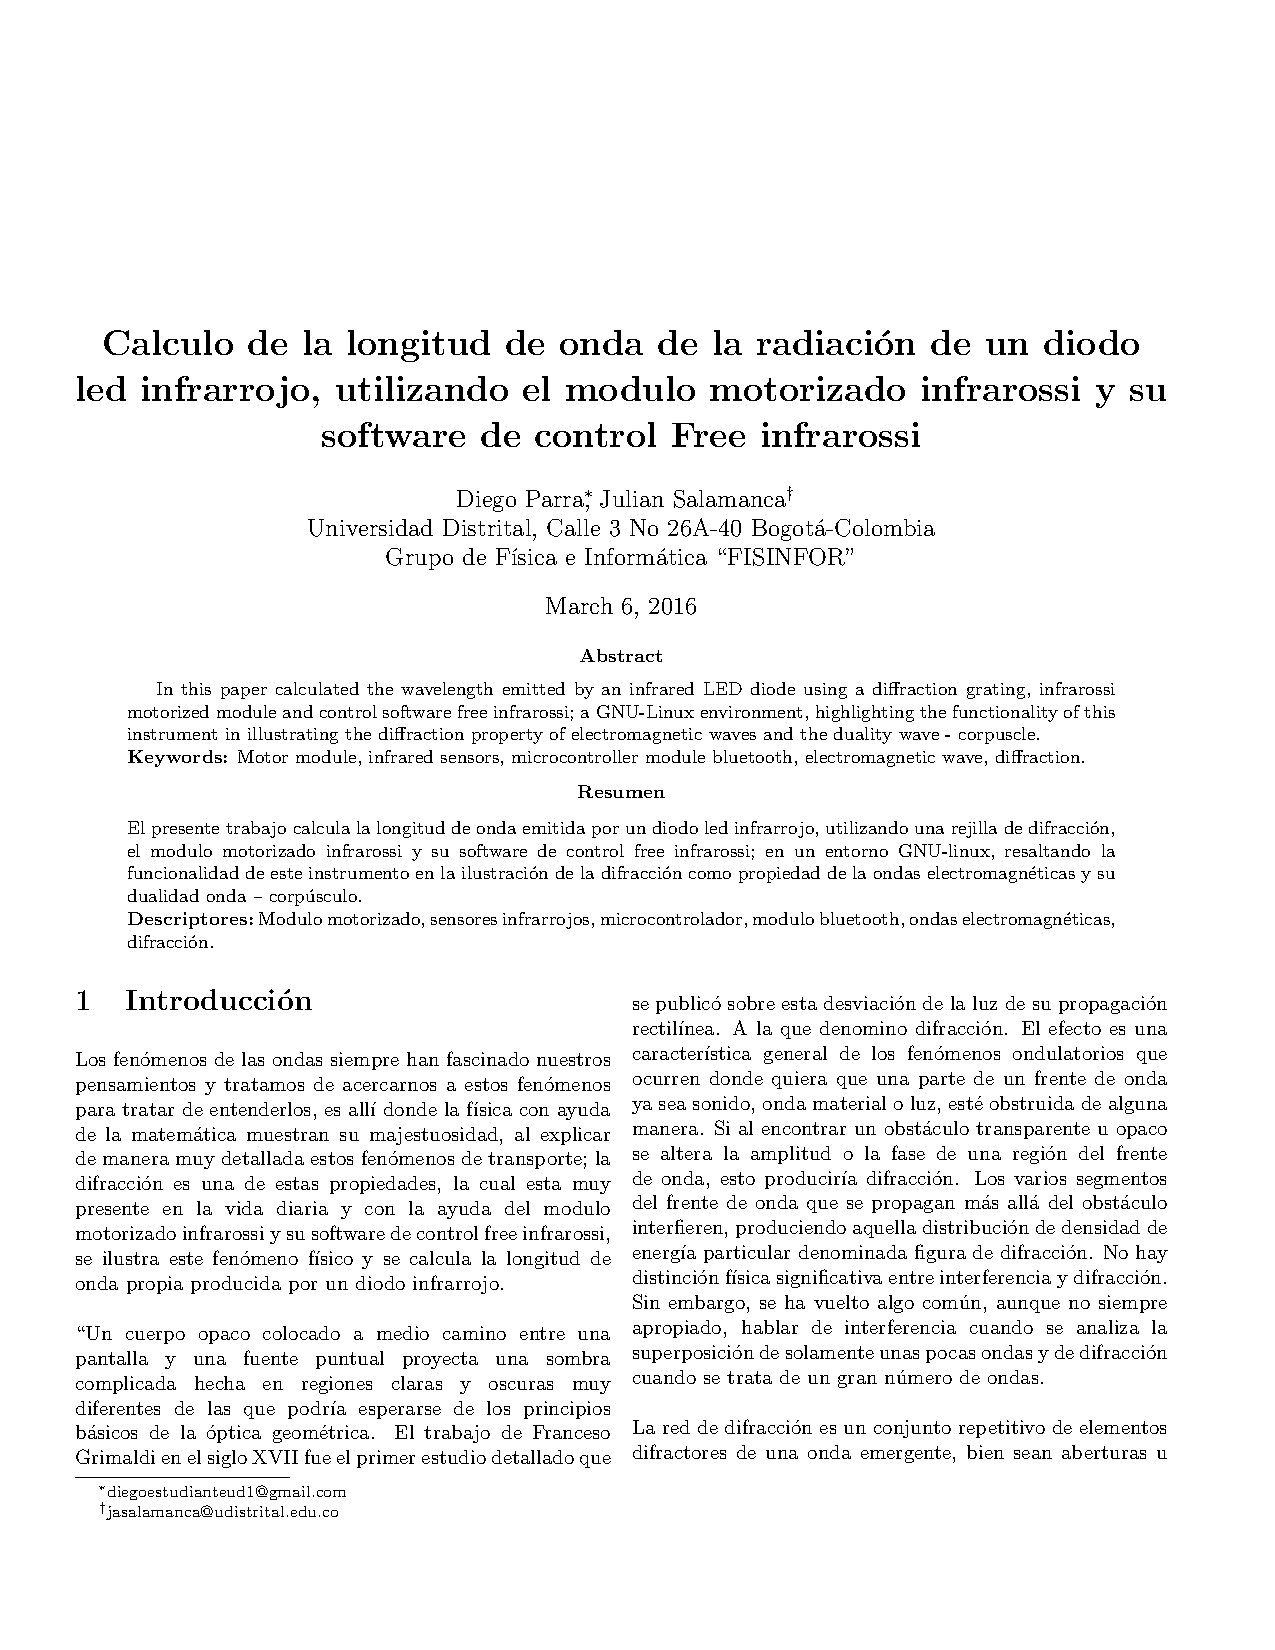
\includepdf[pages=-,scale=1,pagecommand={}]{Articulo_difraccion.pdf}
\subsection{Articulo atenuación}
Este articulo comienza en la pagina que sigue.
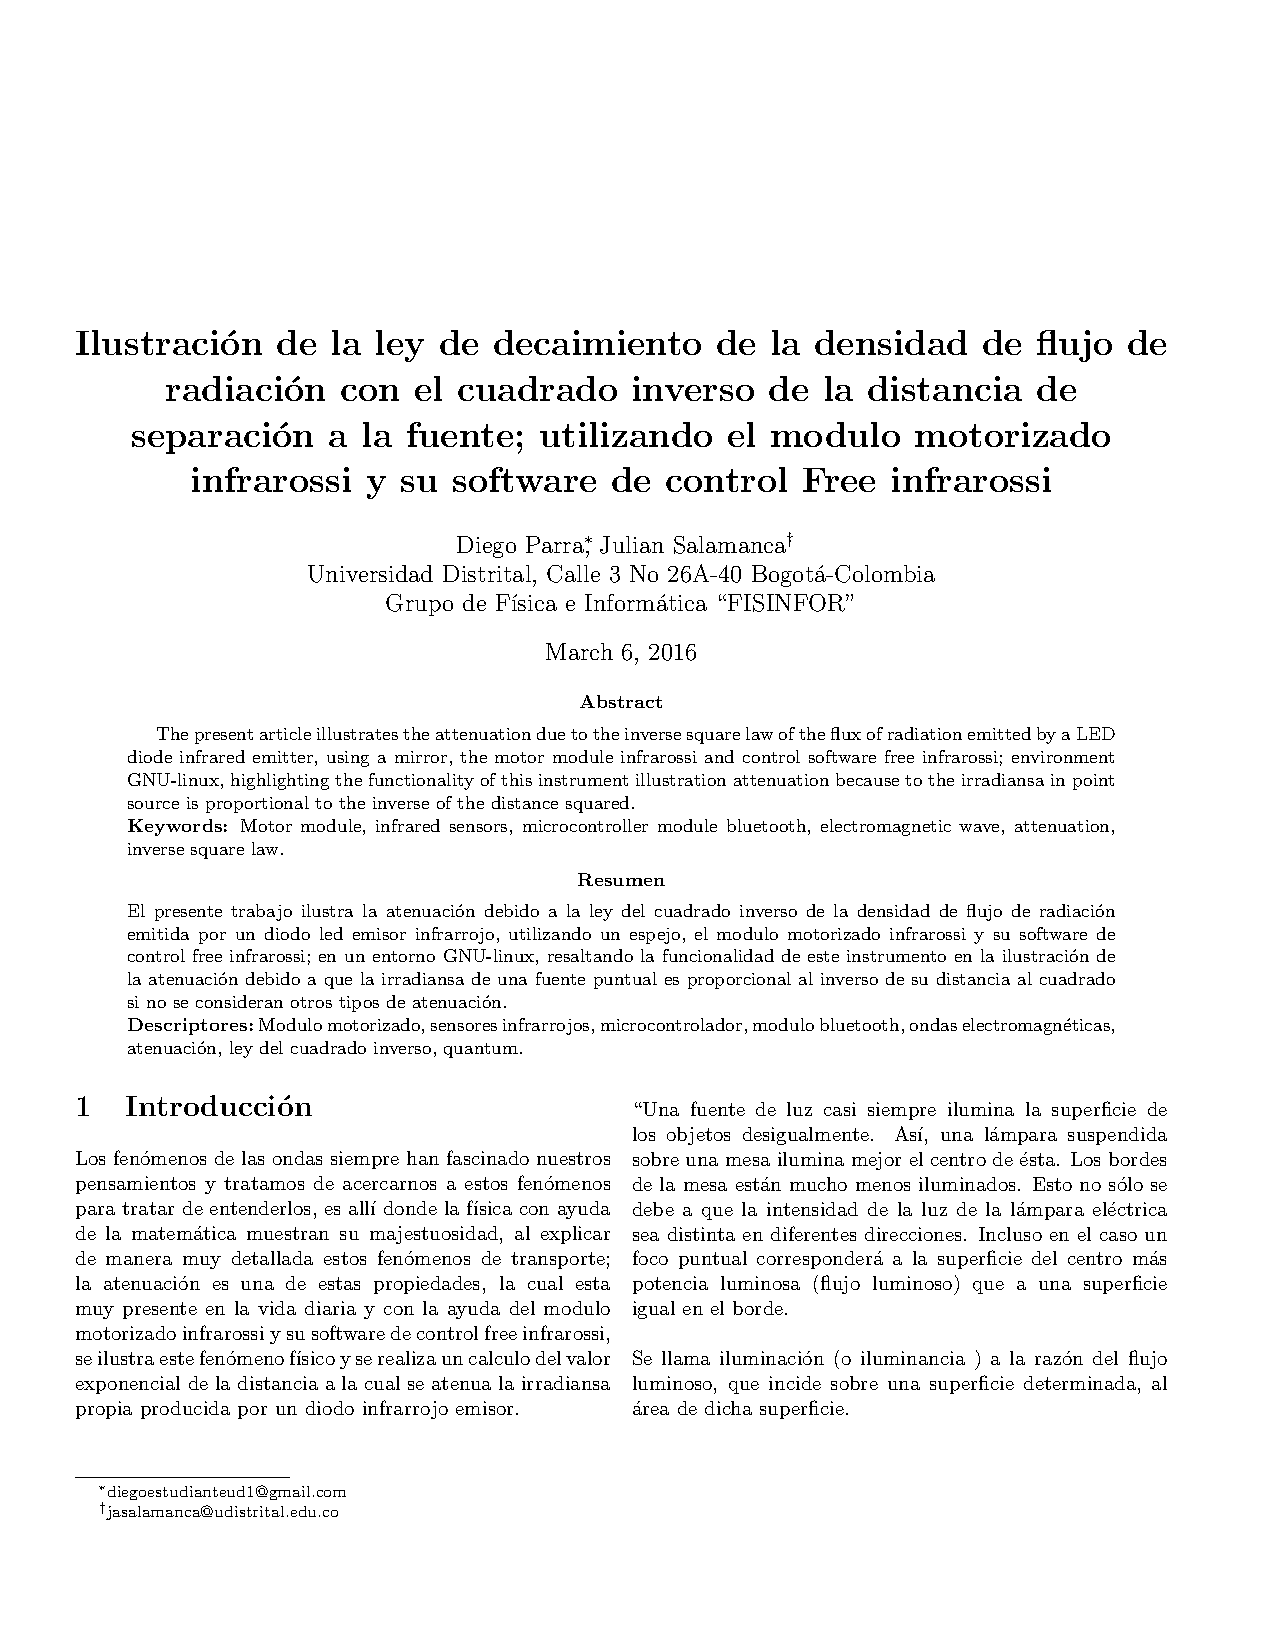
\includepdf[pages=-,scale=1,pagecommand={}]{Articulo_atenuacion.pdf}
\subsection{Articulo absorción}
Este articulo comienza en la pagina que sigue.
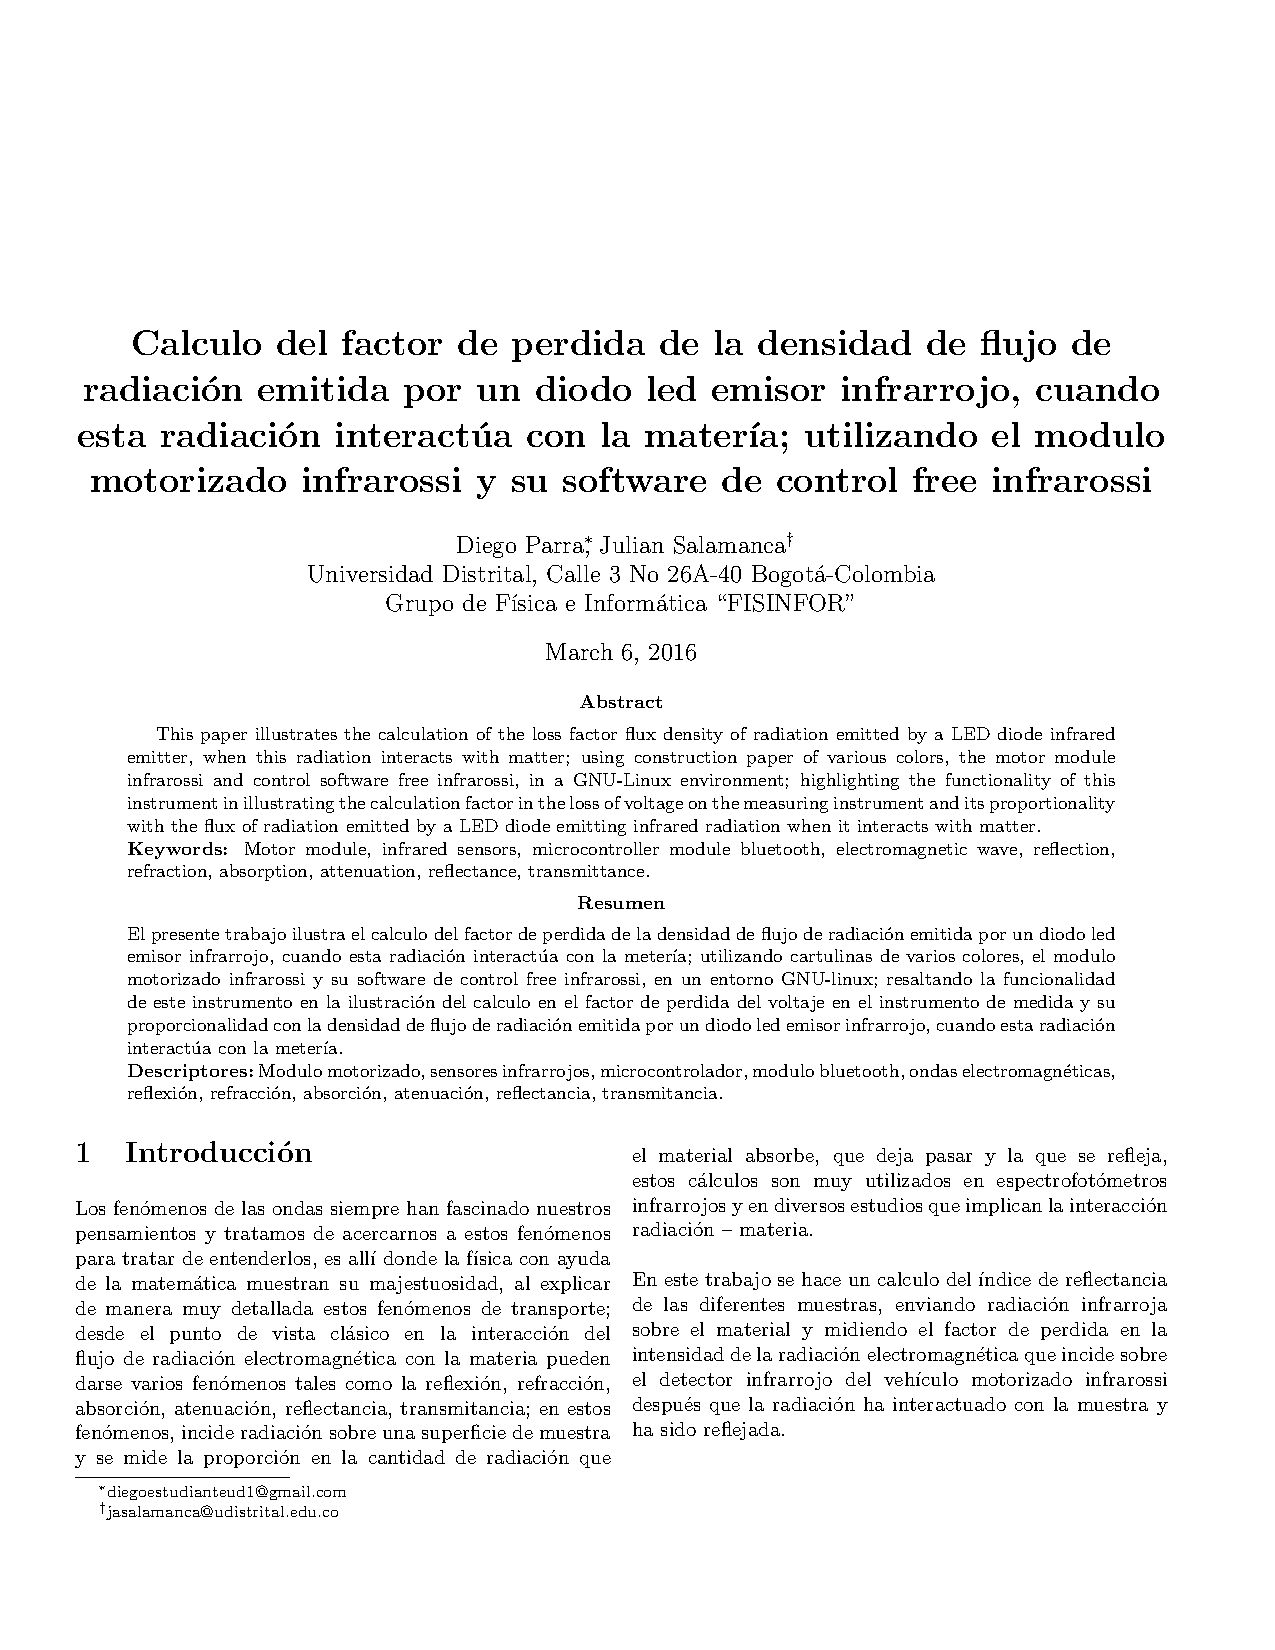
\includepdf[pages=-,scale=1,pagecommand={}]{Articulo_absorcion.pdf}


\end{document}
